\documentclass[11pt,letterpaper]{article}
\usepackage[lmargin=0.9in,rmargin=0.9in,bmargin=0.9in,tmargin=0.9in]{geometry}
\usepackage{style}

\setlength{\parindent}{0ex}

% -------------------
% Content
% -------------------
\begin{document}

% Title 
\begin{center} {\bfseries \Large MATH 122 \par\vspace{0.3cm} \LARGE Exam 1 Review} \end{center} \par\vspace{1cm}


Exam 1 will be selected from the graded and ungraded homeworks on WileyPlus and the problems found below. Problems may be slightly modified, i.e. values in the problem changed, the names or context changed, parts added or removed, plots changed, etc. \pspace

% Problem
\prob Compute the following:
        \begin{enumerate}[(a)]
        \item 36\% of 657.30
        \item 97\% of 450
        \item 154\% of 78.56
        \item 220\% of 11.2
        \end{enumerate} \pspace


% Problem
\prob Compute the following:
        \begin{enumerate}[(a)]
        \item 54 increased by 75\%
        \item 1640 decreased by 22\%
        \item 81 increased by 280\%
        \item 771 decreased by 95\%
        \end{enumerate} \pspace


% Problem
\prob Define $f(x)= 3x - 6$. 
	\begin{enumerate}[(a)]
	\item What type of function is $f(x)$? Explain. 
	\item Without explicitly computing it, find the average rate of change of $f(x)$ on $[-1, 5]$. Explain how you found your answer.
	\item Prove that your answer in (b) is correct. 
	\item Compute $f(17)$.
	\item Is there an $x$ such that $f(x)= 20$? Explain. 
	\end{enumerate} \pspace


% Problem
\prob Is the relation $f(x)= 576.10 - 14.39x$ a function of $x$? Explain. \pspace


% Problem
\prob Is the relation $f(x, y, z)= 45.1x - 36.0y + 1.2z$ a function of $x, y, z$? Explain. \pspace


% Problem
\prob Florist Gump is a floral shop famous for its bouquets. The shop purchases white roses in bulk from their distributor at a price of \$1.42 per rose. The delivery fee for the roses is \$52.50. The shop sells the roses for \$4.32 per rose. 
	\begin{enumerate}[(a)]
	\item Find the revenue function. 
	\item Find the cost function. 
	\item Find the profit function. 
	\item Determine minimal number of white roses the store needs to sell in order to make a profit on their white rose bouquets.
	\end{enumerate} \pspace


% Problem
\prob Let $r(s)= 2s^2 - s + 9$. Compute the following:
	\begin{enumerate}[(a)]
	\item $r(10)$
	\item $r(-1) - r(1)$
	\item The average rate of change of $r(s)$ on $[-3, 8]$. 
	\end{enumerate} \pspace


% Problem
\prob Suppose the barbershop Jack the Clipper has a revenue function and cost functions $R(x)= 0.04x^2 + 23x - 15$ and $C(x)= 5.2x + 3100$, respectively, where $x$ is the number of haircuts given. 
	\begin{enumerate}[(a)]
	\item Find the average revenue, cost, and profit for giving 160 haircuts.
	\item Find the marginal revenue, cost, and profit for giving 160 haircuts. 
	\end{enumerate} \pspace


% Problem
\prob Is the relation shown below a function? Explain. Is the relation shown below linear? Explain. Find the relation plotted below. 
	\[
	\fbox{
	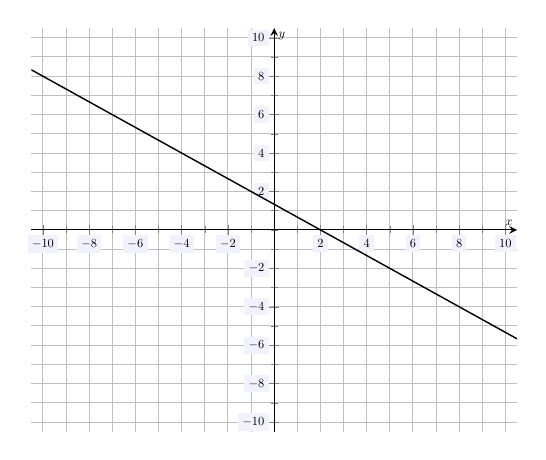
\begin{tikzpicture}[scale=0.9,every node/.style={scale=0.5}]
	\begin{axis}[
	grid=both,
	axis lines=middle,
	ticklabel style={fill=blue!5!white},
	xmin= -10.5, xmax=10.5,
	ymin= -10.5, ymax=10.5,
	xtick={-10,-8,-6,-4,-2,0,2,4,6,8,10},
	ytick={-10,-8,-6,-4,-2,0,2,4,6,8,10},
	minor tick = {-10,-9,...,10},
	xlabel=\(x\),ylabel=\(y\),
	]
	\addplot[line width= 0.02cm,samples=2,domain= -10.5:10.5] ({x},{4/3 - 2/3*x});
	\end{axis}
	\end{tikzpicture}
	}
	\] \pspace


% Problem
\prob Find the equation of the line with $x$-intercept 5 and $y$-intercept $-6$. \pspace


% Problem
\prob A company sells a certain product with associated revenue function $R(x)= 0.14x^2$ and cost function $C(x)= 16x + 530$. 
	\begin{enumerate}[(a)]
	\item Find the fixed costs for this product. 
	\item Find revenue and cost associated to selling and producing 100~units. Is the company making a profit at this level of sales/production? Explain. 
	\item Find the marginal revenue at a production level of 100~units. 
	\end{enumerate} \pspace


% Problem
\prob A company produces widgets. The cost function associated to production is $C(x)= 5x + 120$ and the revenue function for this product is $R(x)= 10x$. 
	\begin{enumerate}[(a)]
	\item What are the fixed costs for production?
	\item How much does each widget cost to produce?
	\item How much does the company sell each widget for?
	\item What is the breakeven point?
	\end{enumerate} \pspace


% Problem 
\prob Consider the linear function $\ell(x)= \frac{13 - 11x}{5}$. 
	\begin{enumerate}[(a)]
	\item Find the slope of this function.
	\item Find the $y$-intercept of this function.
	\item Find the $x$-intercept of this function.
	\item Does the graph of this function contain the point $(6, -8)$? Explain. 
	\end{enumerate} \pspace


% Problem
\prob Showing all your work, compute the following:
	\begin{enumerate}[(a)]
	\item 46\% of 1320
	\item 90\% of 40
	\item 39.6\% of 8476
	\item 1\% of 19.5
	\item 265\% of 210
	\end{enumerate} \pspace
				

% Problem
\prob Suppose that a worker at a local warehouse is paid an hourly wage of \$20/hour. Explain why the worker's net salary is a linear function. \pspace


% Problem
\prob Louise just read \textit{Remembrance of Things Past} by Marcel Proust, which is approximately 3,200~pages long. She kept careful track of the time she was at various pages. She found that she count model the amount of pages she had read, $P$, after $t$ hours by $P(t)= 65t$.
	\begin{enumerate}[(a)]
	\item Find and interpret the slope of $P(t)$.
	\item Find and interpret the $y$-intercept of $P(t)$.
	\item How long did it take her to read this work?
	\end{enumerate} \pspace


% Problem
\prob A certain product requires \$800 of upfront costs to produce---the \textit{fixed costs}. After this investment, it costs \$8.50 to produce each item. 
	\begin{enumerate}[(a)]
	\item Explain why the cost to produce $q$ items, $C(q)$, is a linear function.
	\item Find the equation for $C(q)$.
	\item What does the $y$-intercept for $C(q)$ represent?
	\item How much does it cost to produce 10,000~items?
	\item What is the maximum number of items you could produce with \$6,000?
	\end{enumerate} \pspace


% Problem
\prob You have been saving for a new laptop and printer. You will finally have enough money to purchase them both next month. The laptop costs \$1,899 and the printer costs \$220. Next month, the laptop will go on sale for 5\% less while the printer will be marked up 4\%. The sales tax on the items is 7\%. When you make the purchase of the laptop and printer next month, how much will you pay in total? \pspace


% Problem
\prob Suppose that the revenue and cost function for a certain item are given by $R(q)= 67.99q$ and $C(q)= 13.47q + 495000$, respectively. 
	\begin{enumerate}[(a)]
	\item How much does the company sell each item for? How much does it cost to make each item?
	\item What are the fixed costs for the production of this good?
	\item What is the profit or loss if the company produces and sells ten-thousand of these items?
	\item What is the break-even point? At least many items does this company need to sell in order to make a profit on this item?
	\end{enumerate} \pspace


% Problem
\prob Showing all your work, compute the following:
	\begin{enumerate}[(a)]
	\item 560 increased by 4\%
	\item 357 decreased by 23\%
	\item 993 decreased by 95\%
	\item 55 increased by 105\%
	\item 89.4 increased by 224\%
	\end{enumerate} \pspace


% Problem
\prob A small tanker truck is depositing its gas at a storage facility. The tanker is carrying 11,600~gallons of gas and is emptying its tank at a rate of 528.3~gal/min. Let $G(t)$ denote the volume of gas, in thousands, left in the tanker $t$ minutes from now. 
	\begin{enumerate}[(a)]
	\item Explain why $G(t)$ is linear. 
	\item Find $G(t)$ and sketch it in the plot below. 
	\item Interpret the slope of $G(t)$.
	\item Interpret the $y$-intercept for $G(t)$.
	\item Find and interpret (if possible) the $x$-intercept for $G(t)$. 
	\end{enumerate} \pspace





\newpage





% Problem
\prob Suppose that a company has a revenue function given by $R(q)= 15.8q^2$ and cost function given by $C(q)= 3.1q^2 - 10.8q + 891$, where $q$ is measured in hundreds of items and $R$, $C$ are measured in hundreds of dollars. 
	\begin{enumerate}[(a)]
	\item Find the fixed cost. 
	\item Is the marginal revenue \$15.8 hundreds of dollars per item and the marginal cost \$3.1 hundreds of dollars per item? Explain why or why not. 
	\item Find the average and marginal revenue at a production level of 1,000~items. 
	\item Find the average and marginal cost at a production level of 1,000~items. 
	\item What is the profit at a production level of 1,000~items?
	\end{enumerate} \pspace


% Problem
\prob Spruce Springclean is a cleaning company which offers a basic and deluxe package. The revenue function for $b$ basic cleanings and $d$ deluxe cleanings is $R(b, d)= 45.99b + 69.99d$, while the associated cost function is $C(b, d)= 5.45b + 8.11d + 7.5$. 
	\begin{enumerate}[(a)]
	\item How much does a basic and deluxe cleaning cost? Explain how you know. 
	\item Find the fixed costs.
	\item Find the costs, revenue, and profit for performing 34 basic cleanings and 29 deluxe cleanings. 
	\end{enumerate} \pspace


% Problem
\prob For each of the following, determine the likely dependent variable(s) and independent variable. Then determine, with an explanation, whether the independent variable is a function of the given dependent variable(s). If the independent variable is a function, write it in function notation using appropriate variables. 
	\begin{enumerate}[(a)]
	\item The amount of sales at an electronic store given the number of people that have entered the store since opening. 
	\item The amount of cars that have passed through an intersection some number of hours after 8~am.
	\item The amount of money earned at an hourly job given their hourly pay and hours worked.
	\item The number of children a couple has given their combined income (to the nearest thousand dollars) and the median of their ages. 
	\end{enumerate} \pspace
	

% Problem
\prob Ben and Jerry own an ice cream truck called `The Rolling Cones.' Each day, they drive the truck around the boroughs of NYC trying to satisfy customers in the summer heat. All the standard soft serve flavors sell for the same sale price. Once it is averaged out, the cost of the mixed used to make the cones costs approximately \$0.09 per cone. To turn a profit, they mark-up the cost per cone to \$2.00. However, the cost to run their truck and pay for upkeep, keep their vending license, and pay other associated costs is roughly \$4,235 per month. 
	\begin{enumerate}[(a)]
	\item Find Ben and Jerry's revenue function.
	\item What are Ben and Jerry's variable and fixed costs?
	\item Find Ben and Jerry's cost function. 
	\item What is the minimum number of cones that they must sell each month to turn a profit?
	\end{enumerate} \pspace


% Problem
\prob Consider the following relations below:
	\[
	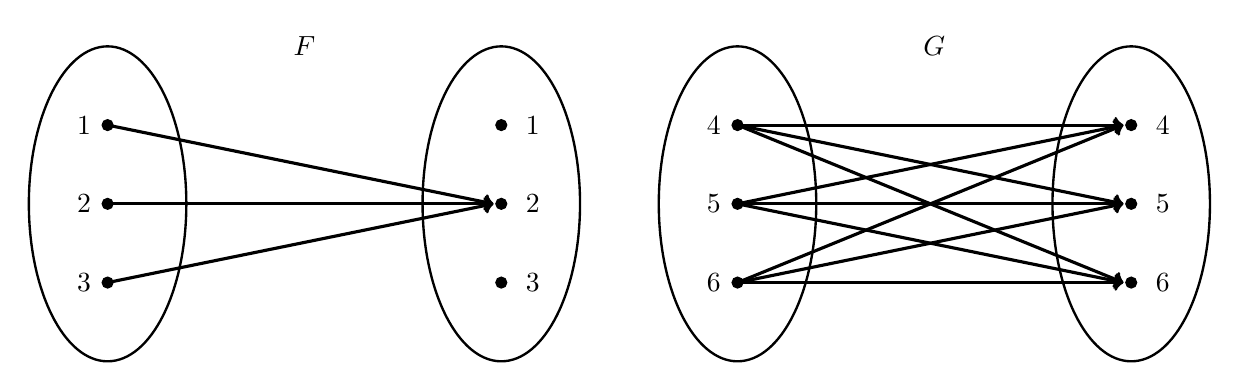
\begin{tikzpicture}
	\node at (2.5,2) {$F$};
	% Ellipses
	\draw[line width=0.03cm] (0,0) circle (1 and 2);
	\draw[line width=0.03cm] (5,0) circle (1 and 2);
	
	% Nodes
	\draw[fill=black] (0,1) circle (0.07);
	\draw[fill=black] (0,0) circle (0.07);
	\draw[fill=black] (0,-1) circle (0.07);
	
	\draw[fill=black] (5,1) circle (0.07);
	\draw[fill=black] (5,0) circle (0.07);
	\draw[fill=black] (5,-1) circle (0.07);
	
	% Arrow
	\draw[line width=0.04cm,->] (0,1) -- (4.9,0);
	\draw[line width=0.04cm,->] (0,0) -- (4.9,0);
	\draw[line width=0.04cm,->] (0,-1) -- (4.9,0);
	
	% Labels
	\node at (-0.3,1) {$1$};
	\node at (-0.3,0) {$2$};
	\node at (-0.3,-1) {$3$};
	
	\node at (5.4,1) {$1$};
	\node at (5.4,0) {$2$};
	\node at (5.4,-1) {$3$};
	
	\tikzset{shift={(8,0)}}
	%
	\node at (2.5,2) {$G$};
	% Ellipses
	\draw[line width=0.03cm] (0,0) circle (1 and 2);
	\draw[line width=0.03cm] (5,0) circle (1 and 2);
	
	% Nodes
	\draw[fill=black] (0,1) circle (0.07);
	\draw[fill=black] (0,0) circle (0.07);
	\draw[fill=black] (0,-1) circle (0.07);
	
	\draw[fill=black] (5,1) circle (0.07);
	\draw[fill=black] (5,0) circle (0.07);
	\draw[fill=black] (5,-1) circle (0.07);
	
	% Arrow
	\draw[line width=0.04cm,->] (0,1) -- (4.9,1);
	\draw[line width=0.04cm,->] (0,1) -- (4.9,0);
	\draw[line width=0.04cm,->] (0,1) -- (4.9,-1);
	\draw[line width=0.04cm,->] (0,0) -- (4.9,1);
	\draw[line width=0.04cm,->] (0,0) -- (4.9,0);
	\draw[line width=0.04cm,->] (0,0) -- (4.9,-1);
	\draw[line width=0.04cm,->] (0,-1) -- (4.9,1);
	\draw[line width=0.04cm,->] (0,-1) -- (4.9,0);
	\draw[line width=0.04cm,->] (0,-1) -- (4.9,-1);
	
	% Labels
	\node at (-0.3,1) {$4$};
	\node at (-0.3,0) {$5$};
	\node at (-0.3,-1) {$6$};
	
	\node at (5.4,1) {$4$};
	\node at (5.4,0) {$5$};
	\node at (5.4,-1) {$6$};
	\end{tikzpicture}
	\] \pspace

	\begin{minipage}[b]{0.49\textwidth}
	\centering
	\begin{tabular}{c|rcc|r}
	$x$ & $H(x)$ & \hspace{1cm} & $x$ & $J(x)$ \\ \cline{1-2} \cline{4-5}
	$1$ & $-1$ & & $5$ & $0$ \\
	$2$ & $2$ & & $6$ & $0$ \\
	$3$ & $3$ & & $8$ & $1$ \\
	$4$ & $-4$ & & $9$ & $0$ \\
	$5$ & $6$ & & $5$ & $1$
	\end{tabular}
	\end{minipage}
	\begin{minipage}[b]{0.49\textwidth}
	\[
	\begin{aligned}
	K(x)&:= 18.87x - 24 \\[0.6cm]
	L(x)&:= 2x(1 - x^8)
	\end{aligned}
	\]
	\end{minipage} \pvspace{0.6cm}
	
Determine if each of the relations given above is a function. \pspace


% Problem
\prob Kent C. Strate is an optometrist would like to save for a down payment on new office space for his business. He deposits a lump sum of \$175,000 into an account that earns 0.43\% annual interest, compounded semiannually. He will move offices in three years. If he uses all the money in this account for his down payment and only this money, what is the largest down payment that he will be able to afford? \pspace


% Problem
\prob Solve the following equation and verify that your solution is correct:
	\[
	9 - 3(x + 1)= \dfrac{6 - x}{2}
	\] \pspace


% Problem
\prob Solve the following equation:
	\[
	5\sqrt{2}\, x + 8= -3(1 - 2x)
	\]  \pspace


% Problem
\prob Determine whether the relations $f(x)= 3x^2 - 4x + 5$ and $g(x, y)= xy^2 - x^2y$ are functions. Be sure to fully justify your answer. Also, find $f(-1)$ and $g(3, -1)$.  \pspace


% Problem
\prob Suppose a company produces two items, $q_1$ and $q_2$, and has a cost function given by $C(q_1, q_2)= 56.20q_1 + 19.45q_2 + 7192$. 
	\begin{enumerate}[(a)]
	\item What are the fixed costs for producing these two items?
	\item What is the total cost associated with producing 30 of the first item and 65 of the second item?
	\item How much does it cost to produce the first item? How much does it cost to produce the second item?
	\end{enumerate} \pspace


% Problem
\prob Monty offers wellness classes at his spa. A session typically costs \$65; however, due to popularity, Monty is raising his prices. Over the next three months, he will raise his prices by 5\% each month. 
	\begin{enumerate}[(a)]
	\item How much will a wellness session cost at the end of the three months? Be sure to justify your answer. 
	\item Is your answer in (a) the same as raising the original price by 15\%? Explain. 
	\item If he simply made the price \$80, by what percentage did he increase the price from the original price?
	\item By what percentage would Monty have to increase his prices over the next three months so that the final cost of a wellness session would be the same as a single price increase of 20\% from the original cost?
	\end{enumerate} \pspace
	
	
% Problem
\prob	 Sue Render wants to be able to save \$500 in the next two years by depositing \$400 in a savings account. She can either choose a savings account that compounds interest quarterly or continuously. For both types of savings account, find the interest rate on the savings account she would have to secure to have the \$500 after 2~years. Does her plan seem feasible? \pspace 
	
	
% Problem
\prob	 Suppose that for a certain product, a company has a revenue given by $R(q)= 53.6q$ and costs given by $C(q)= 228 + 23.7q$, where $q$ is thousands of items and $R$, $C$ are measured in tens of thousands of dollars.
	\begin{enumerate}[(a)]
	\item What are the fixed costs? What are the variable costs?
	\item What is the cost production per item? How much would it cost to product 5,200~items?
	\item How much does the product sell for? What is the revenue yielded by selling 2,000~items?
	\item Find the profit function, $P(q)$.
	\item What is the smallest number of individual units of this product the company must sell to make a profit?
	\end{enumerate} \pspace
	
	
% Problem
\prob	 Suppose you have profit and cost functions given by $R(x)= 95.55x$ and $C(x)= 24.35x + 11450$, respectively. 
	\begin{enumerate}[(a)]
	\item How much does each item sell for? Explain how you know.
	\item What are the fixed costs? Explain how you know.
	\item Find the revenue and costs associated to selling 120~items. Is the seller making a profit?
	\item Sketch $R(x)$, $C(x)$, and $P(x)$ (the profit function) on the same graph---being sure to include the equilibrium point. 
	\end{enumerate} \pspace





\newpage





% Problem
\prob Consider the line given by $f(x)= 6x + 5$.
        \begin{enumerate}[(a)]
        \item Find the $y$-intercept for this line. 
        \item Find the $x$-intercept for this line. 
        \item Is the point $(0, 1)$ on the line? Explain. 
        \item Is the point $(-1, -1)$ on the line? Explain. 
        \end{enumerate} \pspace


% Problem
\prob For each of the following, indicate whether the equation is a linear equation (T), or not (F). 
	\begin{enumerate}[(a)]
	\item  $2x - 3y= 9$
	\item  $2x^2 + 5y^2= 7$
	\item  $x= 5$
	\item  $x= 6- y$
	\item  $y= x^2 + x + 1$
	\end{enumerate} \pspace


% Problem
\prob A fine dining restaurant orders high-quality salmon for their menu. When bought in bulk, each salmon costs \$11.99 and there is a flat delivery fee of \$210. To turn profit on the fish orders, the restaurant marks the price up by 80\%. What is the smallest number of salmon they have to order and sell to make a profit on their salmon sales? \pspace 


% Problem
\prob Aiyana is a statistician. She models that the number of traffic accidents at a particular city intersection can be modeled by $A(c)= 0.002c - 1.3$, where $A$ is the number of accidents and $c$ is the number of cars that pass through the intersection each month. 
	\begin{enumerate}[(a)]
	\item Is the model $A(c)$ linear? Explain.
	\item Find the $y$-intercept for this function. If possible, interpret the intercept in context. 
	\item Find the slope of $A(c)$. If possible, interpret this slope in context. 
	\end{enumerate} \pspace


% Problem
\prob Assume the numbers below represent the slope for some linear function. For each of the given slopes, indicate whether the function is increasing or decreasing and interpret the given slope in at least two different ways:
	\begin{enumerate}[(a)]
	\item $m= 5$
	\item $m= -3$
	\item $m= \dfrac{2}{3}$
	\item $m= -\dfrac{5}{6}$
	\item $m= 4.67$
	\end{enumerate} \pspace


% Problem
\prob Let $C(x)$ be the cost function given by $C(x):= 3.50x + 15$.
        \begin{enumerate}[(a)]
        \item Find the total cost in producing 100 items. 
        \item If the company makes 100 items, what is the average cost of production per item? 
        \item What is the production cost per item? 
        \item Find the $y$-intercept for $C(x)$. 
        \item Interpret your answer from (d). 
        \end{enumerate} \pspace


% Problem
\prob Determine whether the relations $F$ and $G$ shown below are functions. Be sure to fully justify your answer. \pspace
	\hfill
	\begin{minipage}[c]{0.48\textwidth}
	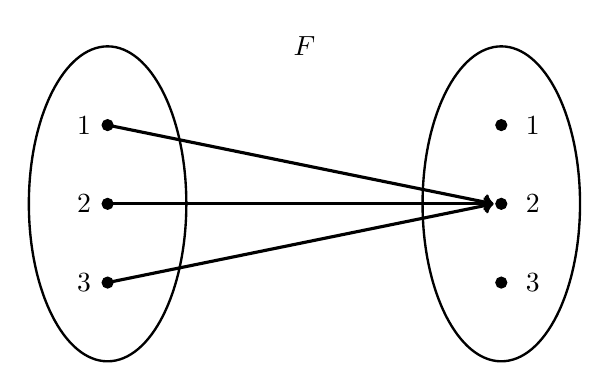
\begin{tikzpicture}
	\node at (2.5,2) {$F$};
	% Ellipses
	\draw[line width=0.03cm] (0,0) circle (1 and 2);
	\draw[line width=0.03cm] (5,0) circle (1 and 2);
	
	% Nodes
	\draw[fill=black] (0,1) circle (0.07);
	\draw[fill=black] (0,0) circle (0.07);
	\draw[fill=black] (0,-1) circle (0.07);
	
	\draw[fill=black] (5,1) circle (0.07);
	\draw[fill=black] (5,0) circle (0.07);
	\draw[fill=black] (5,-1) circle (0.07);
	
	% Arrow
	\draw[line width=0.04cm,->] (0,1) -- (4.9,0);
	\draw[line width=0.04cm,->] (0,0) -- (4.9,0);
	\draw[line width=0.04cm,->] (0,-1) -- (4.9,0);
	
	% Labels
	\node at (-0.3,1) {$1$};
	\node at (-0.3,0) {$2$};
	\node at (-0.3,-1) {$3$};
	
	\node at (5.4,1) {$1$};
	\node at (5.4,0) {$2$};
	\node at (5.4,-1) {$3$};
	\end{tikzpicture}
	\end{minipage}%
	\begin{minipage}[c]{0.40\textwidth}
	\begin{table}[H]
	\centering
	\begin{tabular}{cc}
	$x$ & $G$ \\ \hline
	$1$ & $0$ \\
	$2$ & $2$ \\
	$3$ & $4$ \\
	$4$ & $7$ \\
	$5$ & $0$
	\end{tabular}
	\end{table}
	\end{minipage} \pspace 


% Problem
\prob Suppose $f(x)$ and $g(x)$ are functions. 
	\begin{enumerate}[(a)]
	\item Explain what it means for $f(2)= g(2)$ graphically. 
	\item Explain what $f(x)$ and $g(x)$ intersecting at the point $(-1, 7)$ means algebraically. 
	\end{enumerate} \pspace	
	

% Problem
\prob Suppose that last year, the demand for a certain good was 185~thousand units. It is estimated that next year, the demand will be for 221~thousand units. 
	\begin{enumerate}[(a)]
	\item Assuming that the change in demand is constant, find a linear function predicting the level of demand $t$~years from now.
	\item Interpret the slope and $y$-intercept from your function in (a).
	\item What is your prediction for the level of demand in 5~years?
	\item Predict how many years until the demand is 400~thousand units. 
	\end{enumerate} \pspace


% Problem
\prob Showing all your work, compute the following:
	\begin{enumerate}[(a)]
	\item 78 increased by 40\%
	\item 94 decreased by 65\%
	\item 166 decreased by 2\%
	\item 1820 increased by 163\%
	\end{enumerate} \pspace


% Problem
\prob If you place \$620 in a savings account that earns 1.3\% annual interest, compounded monthly, find the amount that you have after 8~years. \pspace


% Problem
\prob Define $f(x)$ to be the relation given by $f(x):= 2.7x + 14.9$.
	\begin{enumerate}[(a)]
	\item Is $f(x)$ a function? Explain.
	\item Find $f(9)$.
	\item Is there an $x_0$ so that $f(x_0)= 20$? If so, find it. If not, explain why. 
	\item Find the $y$-intercept for $f(x)$. 
	\item Find any $x$-intercepts for $f(x)$.
	\end{enumerate} \pspace


% Problem
\prob Reed wants to buy a tablet for his books while he travels. He finds one that he likes for \$340. Reed places \$240 into an account that earns 1.02\% annual interest, compounded continuously. Assume that he makes no additional deposits. 
	\begin{enumerate}[(a)]
	\item How long until Reed has enough money for the tablet?
	\item How long until Reed would have doubled his money?
	\end{enumerate} \pspace


% Problem
\prob Jordan is taking out a loan for \$13,000. The agreement he negotiates with the bank is for a 5.3\% annual interest rate, compounded continuously. 
	\begin{enumerate}[(a)]
	\item How much will he owe after 5~years?
	\item How much interest will he have been charged on the loan after 5~years?
	\item If he knows that after 5~years he will have at most \$45,000 to pay back on the loan, what is the most he can afford to borrow initially? 
	\end{enumerate} \pspace


% Problem
\prob Being as accurate as possible, sketch the graph of the line $-3x + 5y= 10$.
	\[
	\fbox{
	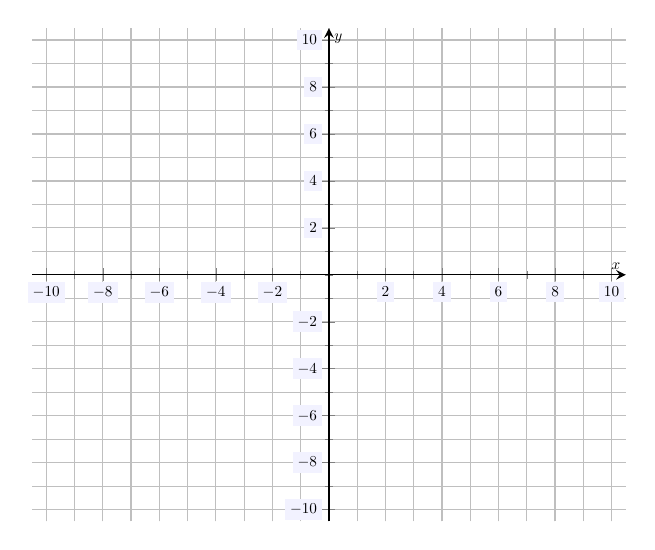
\begin{tikzpicture}[scale=1.1,every node/.style={scale=0.5}]
	\begin{axis}[
	grid=both,
	axis lines=middle,
	ticklabel style={fill=blue!5!white},
	xmin= -10.5, xmax=10.5,
	ymin= -10.5, ymax=10.5,
	xtick={-10,-8,-6,-4,-2,0,2,4,6,8,10},
	ytick={-10,-8,-6,-4,-2,0,2,4,6,8,10},
	minor tick = {-10,-9,...,10},
	xlabel=\(x\),ylabel=\(y\),
	]
	\end{axis}
	\end{tikzpicture}
	}
	\] \pspace 


% Problem
\prob Showing all your work, find the equation of the line with slope $-\frac{1}{3}$ that passes through the point $(9, 4)$. \pspace 


% Problem
\prob The amount of people, on average, that have entered a store $t$~hours after it has opened, $P(t)$, can be modeled by $P(t)= 30.5t - 4$. 
	\begin{enumerate}[(a)]
	\item What does $P(t)$ being linear imply about the rate that people enter the store?
	\item Find and interpret the slope and $y$-intercept of $I(s)$ in context, if possible.
	\item Find $P(2)$ and interpret the value. 
	\item How long after opening until 400~people have entered the store? 
	\end{enumerate} \pspace


% Problem
\prob Determine whether the table of values below could be given by a linear function. If not, explain why. If it can, find the linear function.
        \begin{table}[!ht]
        \centering
        \begin{tabular}{|c || r | r | r |} \hline
	$x$ & $0.2$ & $3.6$ & $5.1$ \\ \hline
	$y$ & $9.84$ & $-1.38$ & $-6.33$ \\ \hline
        \end{tabular}
        \end{table} \pspace


% Problem
\prob Given the following tables, do $f(x)$ and $g(x)$ represent functions? Explain. 
	\begin{table}[!ht]
	\centering \setlength\arrayrulewidth{0.02cm}
	\begin{tabular}{c|ccc|c} 
	$x$ & $f(x)$ & \hspace{2cm} & $x$ & $g(x)$ \\ \cline{1-2} \cline{4-5}
	$1$ & $2$ && $3$ & $3$ \\
	$2$ & $4$ && $4$ & $0$ \\
	$3$ & $6$ && $6$ & $4$ \\
	$4$ & $8$ && $7$ & $5$ \\
	$1$ & $10$ && $8$ & $6$  
	\end{tabular}
	\end{table} \pspace
       

% Problem
\prob Sia Gogh is driving down the highway at 65~mph. She has been driving for 2~hours. Sia determines her total distance traveled $t$~hours from now is approximately $D(t)= 65t + 130$. 
	\begin{enumerate}[(a)]
	\item Explain why her distance traveled is approximately linear.
	\item Interpret the slope of $D(t)$.
	\item Interpret the $y$-intercept of $D(t)$. 
	\item How far has she traveled after a total of 10~hours?
	\end{enumerate} \pspace


% Problem
\prob Two relations, $F$ and $G$, are represented below. Are either $F$ or $G$ functions? Explain. 
	\[
	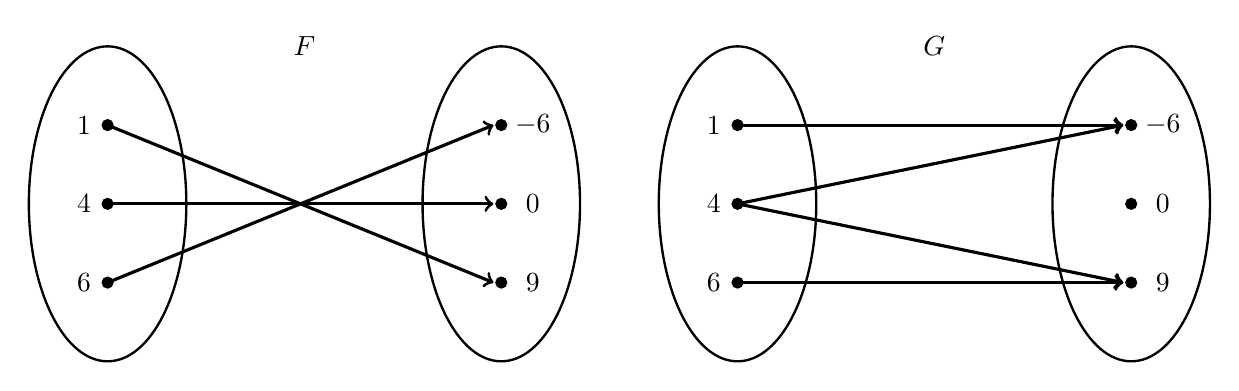
\begin{tikzpicture}
	\node at (2.5,2) {$F$};
	% Ellipses
	\draw[line width=0.03cm] (0,0) circle (1 and 2);
	\draw[line width=0.03cm] (5,0) circle (1 and 2);
	
	% Nodes
	\draw[fill=black] (0,1) circle (0.07);
	\draw[fill=black] (0,0) circle (0.07);
	\draw[fill=black] (0,-1) circle (0.07);
	
	\draw[fill=black] (5,1) circle (0.07);
	\draw[fill=black] (5,0) circle (0.07);
	\draw[fill=black] (5,-1) circle (0.07);
	
	% Arrow
	\draw[line width=0.04cm,->] (0,1) -- (4.9,-1);
	\draw[line width=0.04cm,->] (0,0) -- (4.9,0);
	\draw[line width=0.04cm,->] (0,-1) -- (4.9,1);
	
	% Labels
	\node at (-0.3,1) {$1$};
	\node at (-0.3,0) {$4$};
	\node at (-0.3,-1) {$6$};
	
	\node at (5.4,1) {$-6$};
	\node at (5.4,0) {$0$};
	\node at (5.4,-1) {$9$};
	
	\tikzset{shift={(8,0)}}
	%
	\node at (2.5,2) {$G$};
	% Ellipses
	\draw[line width=0.03cm] (0,0) circle (1 and 2);
	\draw[line width=0.03cm] (5,0) circle (1 and 2);
	
	% Nodes
	\draw[fill=black] (0,1) circle (0.07);
	\draw[fill=black] (0,0) circle (0.07);
	\draw[fill=black] (0,-1) circle (0.07);
	
	\draw[fill=black] (5,1) circle (0.07);
	\draw[fill=black] (5,0) circle (0.07);
	\draw[fill=black] (5,-1) circle (0.07);
	
	% Arrow
	\draw[line width=0.04cm,->] (0,1) -- (4.9,1);
	\draw[line width=0.04cm,->] (0,0) -- (4.9,1);
	\draw[line width=0.04cm,->] (0,0) -- (4.9,-1);
	\draw[line width=0.04cm,->] (0,-1) -- (4.9,-1);
	
	% Labels
	\node at (-0.3,1) {$1$};
	\node at (-0.3,0) {$4$};
	\node at (-0.3,-1) {$6$};
	
	\node at (5.4,1) {$-6$};
	\node at (5.4,0) {$0$};
	\node at (5.4,-1) {$9$};
	\end{tikzpicture}
	\] \pspace
  
  
% Problem
\prob Cheesy Does It is a cheese shop which sells a large variety of cheeses. Suppose they order gouda cheese from a local distributor at a rate of \$5.83 per pound (lb). They are charged a delivery fee of \$87.25 per order. To make a profit selling this cheese, they markup their purchased price by 60\%. 
	\begin{enumerate}[(a)]
	\item Find $C(\ell)$, the costs associated with selling $\ell$ pounds of gouda cheese.
	\item Find $R(\ell)$, the revenue associated with selling $\ell$ pounds of gouda cheese.
	\item Find $P(\ell)$, the profit associated with selling $\ell$ pounds of gouda cheese.
	\item Using $P(\ell)$, find the minimum number of pounds of gouda cheese the store must sell to turn a profit on these cheese sales. 
	\end{enumerate} \pspace 


% Problem
\prob Danisha just started as a sales representative at a local advertising firm. She received a \$1,200 starting bonus and earns \$38/hr. 
	\begin{enumerate}[(a)]
	\item Explain why the amount Danisha has made, $I$, after working at this firm for $d$ days is a linear function.
	\item Assuming Danisha works 8~hour days, find $I(d)$, the amount Danisha has made after working $d$ days at the company. 
	\item Interpret the slope and $y$-intercept from your answer in (b). 
	\item How long until Danisha has earned \$10,000 from working at the company?
	\end{enumerate} \pspace  


% Problem
\prob Howard just started a small business cleaning service called \textit{Grossbusters}. For now, he is renting a truck for \$1,550 per month. On average, he charges \$110 per cleaning and uses approximately \$4.86 in supplies per cleaning. 
	\begin{enumerate}[(a)]
	\item What are the fixed and variable costs for Howard's cleaning service?
	\item Find the cost function for Howard's business.
	\item Find the revenue function for Howard's business.
	\item Find the break-even point for Howard's business. What is the minimal amount of cleanings Howard must book per month to make a profit?
	\item How many cleanings must Howard book each month to make a monthly profit of \$8,000 (translating to a yearly profit of \$96,000)? Does this seem feasible? 
	\end{enumerate} \pspace	  


% Problem
\prob Find the equation of the line containing the point $(-5, 6)$ with slope $-\frac{1}{3}$. \pspace 
  
  
% Problem
\prob An oil company is selling off one of its oil reserves. The amount of oil left in the storage tank in tens of thousands of gallons, $O$, after $d$ days is given by $O(d)= 1600 - 133.4d$.
	\begin{enumerate}[(a)]
	\item Find and interpret the slope of $O(d)$ in the context of the problem.
	\item Find and interpret the $y$-intercept of $O(d)$ in the context of the problem.
	\item Find how long it will take the company to sell all the oil in the tank. 
	\item If the company sells the oil for \$2.085/gallon, how much money do they make selling this reserve oil?
	\end{enumerate} \pspace


% Problem
\prob Consider the revenue function, $R(q)$, and cost function, $C(q)$, for some good given in the plot below. 
	\[
	\fbox{
	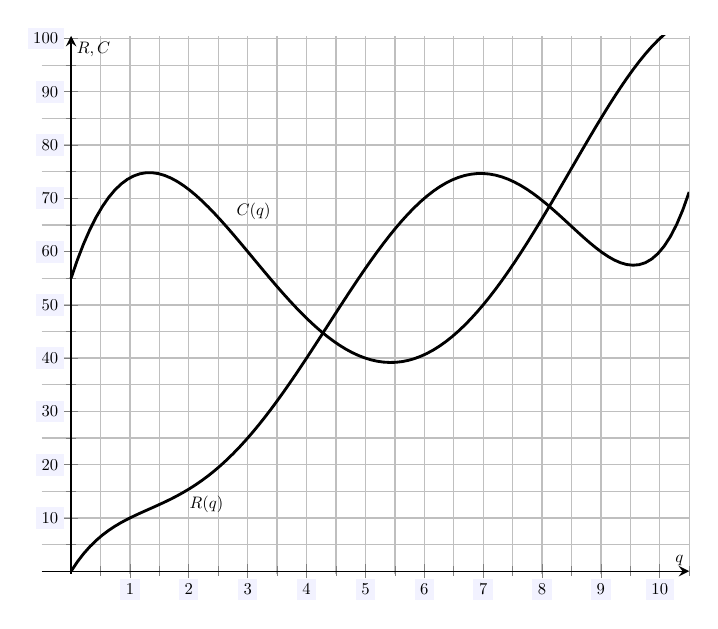
\begin{tikzpicture}[scale=1.2,every node/.style={scale=0.5}]
	\begin{axis}[
	grid=both,
	axis lines=middle,
	ticklabel style={fill=blue!5!white},
	xmin= -0.5, xmax=10.5,
	ymin= -0.5, ymax=100.5,
	xtick={0,1,2,...,11},
	ytick={0,10,20,...,100},
	minor x tick num = 1,
	minor y tick num = 1,
	xlabel=\(q\),ylabel=\({R,C}\),
	]
	\node at (2.3,12.5) {$R(q)$};
	\addplot[domain=0:10.5, samples=100,line width=0.03cm] 
	(x, 17.6667*x - 11.3056*x^2 + 4.16204*x^3 - 0.546296*x^4 + 0.0231481*x^5);
	\node at (3.1,67.5) {$C(q)$};
	\addplot[domain=0:10.5, samples=100,line width=0.03cm] 
	(x, 55 + 33.994*x - 17.7014*x^2 + 2.69544*x^3 - 0.131944*x^4 + 0.000992063*x^5);
	\end{axis}
	\end{tikzpicture}
	}
	\] 
In the plot above, the number of goods produced, $q$, is measured in tens of thousands of items and the outputs of $R(q)$ and $C(q)$ are measured in tens of thousands of dollars. Given this data, answer the following:
	\begin{enumerate}[(a)]
	\item What are the fixed costs?
	\item What the break-even point(s)?
	\item Is the company experiencing profit or loss for this good at a production level of 65,000~units?
	\item Estimate the profit or loss in (c). 
	\item  Estimate the average revenue per sale at a production/sale level of 70,000~units. 
	\end{enumerate} \pspace  


% Problem
\prob Values for several functions are given in the table below. 
        \begin{table}[!ht]
        \centering
        \begin{tabular}{| c || c | c | c | c | c | c | c |} \hline
	$x$ & $-3$ & $-2$ & $-1$ & $\phantom{-}0$ & $\phantom{-}1$ & $\phantom{-}2$ & $\phantom{-}3$ \\ \hline \hline
	$f(x)$ & $\phantom{-}4$ & $8$ & $-1$ & $\phantom{-}5$ & $-3$ & $\phantom{-}0$ & $-2$ \\ \hline
	$g(x)$ & $\phantom{-}1$ & $6$ & $\phantom{-}0$ & $-6$ & $-7$ & $-3$ & $\phantom{-}1$ \\ \hline
	$h(x)$ & $-4$ & $0$ & $\phantom{-}3$ & $\phantom{-}5$ & $10$ & $\phantom{-}3$ & $\phantom{-}9$ \\ \hline
        \end{tabular}
        \end{table}

Given the data above, compute the following: 
        \begin{enumerate}[(a)]
        \item $(h + g)(-2)=$ 
        \item $(f - g)(0)=$ 
        \item $(5h)(1)=$ 
        \item $\left(\dfrac{h}{f}\right)(1)=$ 
        \item $g(-3)\, h(3)=$ 
        \item $g \big(-1 - f(3) \big)=$ 
        \item $(h \circ g)(2)=$ 
	\item $(g \circ h)(2)=$ 
        \item $(f \circ g)(-1)=$ 
	\item $(h \circ g \circ f)(1)=$ 
        \end{enumerate} \pspace  
  
  
% Problem
\prob Jeff is arguing with Carol. Over the last 7~months, the cost of products has risen 4\% each month. Jeff then argues that goods now cost $7 \cdot 4\%= 28\%$ more now than they cost 4~months ago. Carol claims that this is not correct and that goods now cost a little more than 30\% more than they did 7~months ago. Who is correct? Be sure to fully justify your response. \pspace 
  
  
% Problem
\prob Explain why $f(x, y)= 2x^2 - y^3 + 6$ is a function. Then find $f(0, 0)$, $f(3, -1)$, $f(-3, 2)$, and $f(1, 1)$. \pspace 
  

% Problem
\prob Determine if the relations $f(x)$ and $g(x)$ shown below are functions. Explain why or why not. If the relation is a function, compute the functions value at $x= -4.1$. 
	\[
	\begin{aligned}
	f(x)&= 198.3 - 17.3x \\[0.3cm]
	g(x)&= 4x^2 + 16.1x - 10.3
	\end{aligned}
	\] \pspace	      
       
  
% Problem
\prob Consider the linear function $f(x)= 7 - \frac{6}{7}\, x$.
	\begin{enumerate}[(a)]
	\item Find the rate of change of $f(x)$.
	\item Is $f(x)$ increasing or decreasing? Explain.
	\item Find the $y$-intercept of $f(x)$.
	\item Find $f(-3)$.
	\end{enumerate} \pspace  
  
  
% Problem
\prob Plot the function $f(x):= \frac{1}{2}x - 5$, being as accurate as possible. 
	\[
	\fbox{
	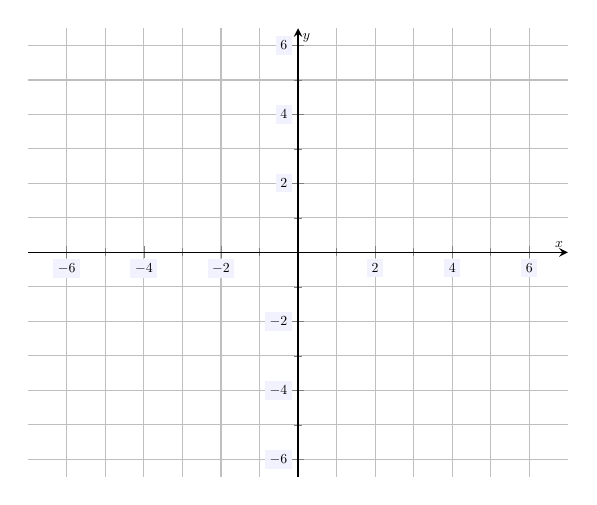
\begin{tikzpicture}[scale=1.0,every node/.style={scale=0.5}]
	\begin{axis}[
	grid=both,
	axis lines=middle,
	ticklabel style={fill=blue!5!white},
	xmin= -7, xmax=7,
	ymin= -6.5, ymax=6.5,
	xtick={-6,-4,-2,0,2,4,6},
	ytick={-6,-4,-2,0,2,4,6},
	minor tick = {-5,-3,...,5},
	xlabel=\(x\),ylabel=\(y\),
	]
	\end{axis}
	\end{tikzpicture}
	}
	\] \pspace  


% Problem
\prob Inna Vesta Moore places \$7,800 of her savings into a savings account that earns 0.57\% annual interest, compounded monthly. 
	\begin{enumerate}[(a)]
	\item How much will be in the account after 9~years?
	\item How much interest has the account earned after 9~years?
	\item How long would it take the account to have \$50,000?
	\end{enumerate} \pspace
  


% Problem
\prob You keep a secret lunchbox under your bed filled with cash. The lunchbox currently contains \$2,500. Each week, you place \$80 into the lunchbox. Let $M(w)$ denote the amount of money in the lunchbox $w$~weeks from now. 
	\begin{enumerate}[(a)]
	\item Explain why $M(w)$ is linear.
	\item Find $M(w)$. 
	\item Use (b) to find how long until the lunchbox has \$10,000. 
	\end{enumerate} \pspace
	
	
% Problem
\prob Leslie owns a wine and spirit store called \textit{Planet of the Grapes}. She rents the building for \$24,730 per month. The average bottle of wine or spirit at her store sells for \$11.56. The average cost of ordering, stocking, and selling these wines/spirits is \$5.21 per bottle. 
	\begin{enumerate}[(a)]
	\item What are the fixed and variable costs for Leslie's business?
	\item Find the cost function for Leslie's business.
	\item Find the revenue function for Leslie's business.
	\item Find the break-even point for Leslie's business. 
	\item What is the minimal average amount of bottles Leslie must sell per month to make a profit?
	\item How many bottles must Leslie sell each month on average to make a profit of \$15,000 (translating to a yearly profit of \$180,000)? Does this seem feasible?	
	\end{enumerate} \pspace	
	

% Problem
\prob An investment firm promises that if you place your money with them that you will see returns of 9.7\% annual interest, compounded semiannually. You decide to place \$86,000 with this firm. 
	\begin{enumerate}[(a)]
	\item How long until your investment is worth \$100,000?
	\item If instead they claimed the return was 9.7\% annual interest, compounded continuously, how long until your investment would be worth \$100,000?
	\item Why is your answer in (b) a shorter time period than your answer in (a)?
	\end{enumerate} \pspace	
	

% Problem
\prob Petra Fried has taken out a \$27,000 loan with a bank to go in on a business called `Amy's Winehouse' with her friend Amy. The bank charges Petra 8.91\% annual interest, compounded continuously. 
	\begin{enumerate}[(a)]
	\item How much will Petra owe the bank after 2~years?
	\item How long until Petra owes the bank \$50,000? 
	\end{enumerate} \pspace	
	

% Problem
\prob You are driving back to college after summer break. It is 12~pm and you are traveling on the highway at a constant speed of 65~mph. Currently, you are 211~mi from college. Let $D(t)$ denote your distance, in miles, that you are from the college $t$ hours from now. 
	\begin{enumerate}[(a)]
	\item Explain why $D(t)$ is linear.
	\item Find $D(t)$. 
	\item What do the slope and $y$-intercept of $W(t)$ represent in context?
	\item Determine when you will arrive at the college. 
	\end{enumerate} \pspace 	
	
	
% Problem
\prob A certain species of fungus reproduces by releasing tiny spores. The larger the fungus, the more spores that are released. Scientists find that the number of spores (in thousands) a fungus with diameter $d$ (in inches) can be modeled by $N(d)= -3.5 + 15.5d$.
	\begin{enumerate}[(a)]
	\item Find and interpret the slope of $N(d)$ in the context of the problem.
	\item Find and interpret in the context of the problem, if possible, the $y$-intercept of $N(d)$.
	\item According to the model, how large would the fungus have to be in order for it to release 100,000 spores?
	\end{enumerate} \pspace	
	

% Problem
\prob	 Consider the line $2x - 5y= 4$.
	\begin{enumerate}[(a)]
	\item Is $(-2, 0)$ on the line? Explain.
	\item Is $(-3, -2)$ on the line? Explain.
	\item Showing all your work, find two points, distinct from $(-2, 0)$ and $(-3, -2)$, on the given line. 
	\end{enumerate} \pspace


% Problem
\prob Solve the following equation and check your solution:
	\[
	\dfrac{x - 3}{1 - x}= 5
	\] \pspace
	
	
% Problem
\prob Thai Tanic is a new restaurant chain that has been expanding across the Northwest. It is projected that next year, it will have \$800,000 in profits and the following year it will have \$1.2~million in profits. 
	\begin{enumerate}[(a)]
	\item Under what assumptions is a linear model to predict the growth rate of this business appropriate?
	\item Find a linear model for the profit of this company $t$ years from today. 
	\item Interpret the slope of your linear model in (b).
	\item Interpret the $y$-intercept of your linear model in (b), if possible. 
	\item How long until the company has a profit of \$5~million? 
	\end{enumerate} \pspace		
	
	
% Problem
\prob Jeffrey is writing a term paper. Currently, he has only written 8~pages. He returns from a writing break and then goes back to the paper. After an additional 5~hours of writing, he has written 20~pages. 
	\begin{enumerate}[(a)]
	\item Assuming Jeffrey writes at a constant rate, find the linear function representing the number of pages that he has written after $t$ hours of writing. 
	\item How long after this break will it take him in total to write this 50~page term paper?
	\end{enumerate} \pspace 	


% Problem
\prob Consider the relation plotted below:
	\[
	\fbox{
	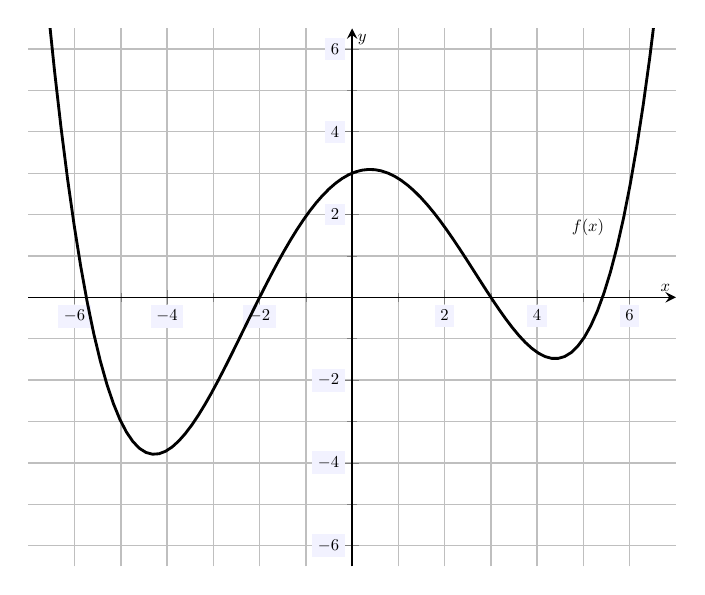
\begin{tikzpicture}[scale=1.2,every node/.style={scale=0.5}]
	\begin{axis}[
	grid=both,
	axis lines=middle,
	ticklabel style={fill=blue!5!white},
	xmin= -7, xmax=7,
	ymin= -6.5, ymax=6.5,
	xtick={-6,-4,-2,0,2,4,6},
	ytick={-6,-4,-2,0,2,4,6},
	minor tick = {-5,-3,...,5},
	xlabel=\(x\),ylabel=\(y\),
	]
	\addplot[domain=-7:7, samples=100,line width=0.03cm] (x,3+0.467857*x-0.601786*x^2-0.0107143*x^3+0.0160714*x^4);
	\node at (5.1,1.7) {$f(x)$};
	\end{axis}
	\end{tikzpicture}
	}
	\]

\begin{enumerate}[(a)]
\item Is the relation, $f(x)$, plotted above a function? Explain. 
\item Find the $y$-intercept.
\item Find the $x$-intercepts. 
\item Find the value of $f(6)$.
\item Find any $x$-values for which $f(x)= 2$.  
\end{enumerate} \pspace


% Problem
\prob Annita needs a loan. After discussing with a loan officer, she is offered a loan with an annual interest rate of 11.43\%, compounded monthly. 
	\begin{enumerate}[(a)]
	\item What is the nominal interest rate?
	\item What is the effective interest rate for this loan?
	\item If Annita will take out the loan for 4~years and will not be able to pay back more than \$11,000, what is the most she can take out now? That is, what is the amount that she could borrow now so that after 4~years, she would owe \$11,000?
	\end{enumerate} \pspace	


% Problem
\prob Without explicitly finding the intersection, explain why the following lines $y= 2(7 - 5x)$ and $y= 5x + 2$ intersect. Showing all your work, find the intersection of the lines. \pspace 	





\newpage





% Problem
\prob For each of the following, describe whether the given dependent variable is a function of the independent variable:
	\begin{enumerate}[(a)]
	\item Independent: the number of days since you purchased your car. \par 
		Dependent: the milage for your car. 
	\item Independent: the number of people in a specific room at noon. \par 
		Dependent: the day of the week.
	\item Independent: the day of the year. \par
		Dependent: the sunrise time. 
	\item Independent: your laptop battery percentage. \par
		Dependent: the time remaining until your laptop runs out of power. 
	\end{enumerate} \pspace


% Problem
\prob Suppose that you have a revenue function given by $R(q)= 89q$ and a cost function given by $C(q)= 45q + 7200$. 
	\begin{enumerate}[(a)]
	\item What are the revenue and cost at a production/sale level of 60~units?
	\item Without finding the profit function, find the break-even point for the production/sale of this item.
	\item Find the profit function, $P(q)$.
	\item Compute $P(60)$. Explain how you could use (a) to find $P(60)$. 
	\end{enumerate} \pspace


% Problem
\prob Consider the line $4x - 6y= 12$.
	\begin{enumerate}[(a)]
	\item Determine the slope of the given line.
	\item Interpret the slope in at least two different ways.
	\item Is the function whose graph is the given line an increasing or decreasing function? Explain. 
	\item Determine the $y$-intercept of the given line. 
	\item Determine the $x$-intercept of the given line. 
	\end{enumerate} \pspace		


% Problem
\prob Consider the linear function $f(x)= 7 - \frac{6}{5}\,x$. Showing all your work, answer the following:
	\begin{enumerate}[(a)]
	\item Find the rate of change of $f(x)$.
	\item Interpret the rate of change of $f(x)$. 
	\item Determine whether $f(x)$ is an increasing or decreasing function.
	\item Determine the $y$-intercept of $f(x)$.
	\item Find the exact value of $f \big( \frac{2}{3} \big)$. 
	\end{enumerate} \pspace





\newpage





% Problem
\prob Consider the line $-3x - 5y= 10$.
	\begin{enumerate}[(a)]
	\item Find the slope of the line.
	\item Find the $y$-intercept of the line.
	\item Find this line as a linear function, $f(x)$.
	\item Using your $f(x)$ from (c), find a point on the line distinct from the $y$-intercept.
	\end{enumerate} \pspace  


% Problem
\prob Suppose $f(x)$ and $g(x)$ are the functions given below. 
	\[
	\begin{aligned}
	f(x)&= 2x - 3 \\[0.3cm]
	g(x)&= x^2 + 2x - 1
	\end{aligned}
	\]

Compute the following: \pspace
        \begin{enumerate}[(a)]
        \item $f(5)=$ 
        \item $g(-2)=$ 
        \item $f(0) - 3g(2)=$ 
        \item $(f - g)(x)=$ 
        \item $(fg)(x)=$ 
        \item $\left( \dfrac{f}{g} \right)(x)=$ 
        \item $(f \circ g)(0)=$ 
        \item $(g \circ f)(0)=$ 
        \item $(f \circ g)(x)=$ 
        \item $(g \circ f)(x)=$ 
        \end{enumerate} \pspace  


% Problem
\prob For each of the following, describe whether the given dependent variable is a function of the independent variable:
	\begin{enumerate}[(a)]
	\item Independent: Number of stains removed by a test detergent. 
		Dependent: Type of detergent used. 
	\item Independent: Time since the song began.
		Dependent: Number of words spoken in the song. 
	\item Independent: Phase of the moon.
		Dependent: Day of the week. 
	\item Independent: Number of days since an account was opened. 
		Dependent: Amount of money in the account. 
	\end{enumerate} \pspace


% Problem
\prob Emma Minat needs some quick cash by the end of next year to help fund her growing addiction to soap carving. She estimates that she will need at least \$8,500 to fund her newest series of soapy endeavors. Emma finds a new type of bond that offers 3.35\% annual interest, compounded weekly. 
	\begin{enumerate}[(a)]
	\item How much should she take out in these bonds to have the necessary \$8,500 by the end of the two years?
	\item How much longer would Emma have to let these bonds accrue interest before they are worth \$10,000?
	\end{enumerate} \pspace  


% Problem
\prob Piper is tired of her parents yelling at her to start saving for college---mostly because she wants to be a TikTok prank influencer. However, to quell their complaints, she starts setting aside money from her job to save for college textbooks. If she were to go to college, she estimates that she would spend at least \$600 each semester of college on textbooks. 
	\begin{enumerate}[(a)]
	\item What is the minimum amount she should estimate that she will spend on books while in college? 
	\item How much should she deposit into an account earning 1.17\% annual interest, compounded quarterly, so that she will have the minimum amount she estimated in (a) that she would need for college textbooks after 5 years? 
	\end{enumerate} \pspace  
  
  
% Problem
\prob Suppose that the revenue and cost function for a certain item are given by $R(q)= 45.99q$ and $C(q)= 11.13q + 576000$, respectively. 
	\begin{enumerate}[(a)]
	\item How much does the company sell each item for? How much does it cost to make each item?
	\item What are the fixed costs for the production of this good?
	\item What is the profit or loss if the company produces and sells ten-thousand of these items?
	\item What is the break-even point? At least many items does this company need to sell in order to make a profit on this item?
	\end{enumerate} \pspace


% Problem
\prob Sue Flay is taking out a small business loan to open her dream bakery. The loan she takes out is for \$85,000 at a 2.89\% annual interest rate, compounded monthly.
	\begin{enumerate}[(a)]
	\item What is the effective interest rate for this loan?
	\item How much does she owe after 2~years?
	\item How long until Sue owes the bank \$150,000?
	\end{enumerate} \pspace


% Problem
\prob Ray runs a vegetable stand called `Beets by Ray.' The radishes he sells cost him an average of \$0.86 per radish in production costs. In order to turn a profit on their sale, he marks them up by 89.5\%.
	\begin{enumerate}[(a)]
	\item Find the amount by which Ray increases the beet price.
	\item Using your answer from (a), find the price at which he markets the beets.
	\item By recognizing the market price of the beets as a percent increase problem, find the market price of the beets you found in (b) `directly.'
	\item If a customer that purchases 36~beets from Ray and must pay a 7\% tax, what is the final purchase price?
	\end{enumerate} \pspace


% Problem
\prob Brock Lee is open a savings account to have enough money for community college. He places \$2,500 in the account, which earns 0.13\% annual interest, compounded continuously.
	\begin{enumerate}[(a)]
	\item What is the effective interest rate for this account?
	\item How much is in his account after 4~years?
	\item If the cost of a year at the college is \$21,714, how much should have Lee placed in the account to have enough for his first full year at the college in four years?
	\end{enumerate} \pspace


% Problem
\prob Suppose that you have a revenue function given by $R(q)= 120q$ and a cost function given by $C(q)= 70q + 1600$. 
	\begin{enumerate}[(a)]
	\item What are the revenue and cost at a production/sale level of 80~units?
	\item Without finding the profit function, find the break-even point for the production/sale of this item.
	\item Find the profit function, $P(q)$.
	\item Compute $P(80)$. Explain how you could use (a) to find $P(80)$. 
	\end{enumerate} \pspace


% Problem
\prob Braden Haire is investing some of the profits from his politically active wig company Wigs for Whigs. He places \$65,000 into an account that advertises a 4.15\% annual interest rate, compounded continuously. 
	\begin{enumerate}[(a)]
	\item One year from now, by what percentage would Braden's money have increased?
	\item Assuming Braden makes no additional deposits into the account, how much will be in the account after 33~years?
	\item How much interest would the account have earned after 33~years?
	\end{enumerate} \pspace


% Problem
\prob A laptop from Macrosoft is advertised as being \$999. You plan on ordering this computer online. You know that you will be charged 7\% sales tax. How much will the computer then cost? If you find out that the laptop costs Macrosoft \$89 to produce, what is the percent markup that Macrosoft puts on this laptop? How much profit do they make per laptop? \pspace 


% Problem
\prob Give an example of a `real world' relationship between two variables which does represent a functional relationship. Also, give an example of a `real world' relationship between two variables which \textit{does not} represent a functional relationship. Be sure to fully explain your responses. \pspace 


% Problem
\prob Suppose $f(x)$ and $g(x)$ are the functions given below. 
	\[
	\begin{aligned}
	f(x)&= 2 - x \\[0.3cm]
	g(x)&= x^2 - 3x + 2
	\end{aligned}
	\]

Compute the following: 
        \begin{enumerate}[(a)]
        \item $f(-4)=$ 
        \item $g(2)=$ 
        \item $2f(1) - g(3)=$ 
        \item $f(x) - g(x)=$ 
        \item $f(x) \, g(x)=$ 
        \item $\left( \dfrac{f}{g} \right)(x)=$ 
        \item $(f \circ g)(0)=$ 
        \item $(g \circ f)(0)=$ 
        \item $(f \circ g)(x)=$ 
        \item $(g \circ f)(x)=$ 
        \end{enumerate} \pspace 


% Problem
\prob If $f(x)= 5 - 3x$ and $g(x)= -3(x + 8)$, will there be a solution to $f(x)= g(x)$? Explain. \pspace 


% Problem
\prob Showing all your work, find the solution to the following:
	\[
	2(x - 9)= \frac{x}{3} + 7
	\] \pspace


% Problem
\prob Showing all your work, find the following:
	\begin{enumerate}[(a)]
	\item 56\% of 920
	\item 150\% of 60
	\item 1\% of 840
	\end{enumerate} \pspace

% Problem
\prob Find the equation of the line passing through the points $(-5, 8)$ and $(7, 8)$. \pspace 


% Problem
\prob A product has cost function $C(q)= 12.67q + 16200$ and revenue function $R(q)= 29.99q$. 
	\begin{enumerate}[(a)]
	\item What are the fixed costs? 
	\item How much does it cost to produce each product? How much does each product sell for?
	\item Find the break-even point.
	\item What is the minimum number of items that must be made/sold in order to make a profit?
	\end{enumerate} \pspace


% Problem
\prob Find the linear function through the points $(-1, 6)$ and $(3, -4)$. Is this linear function increasing or decreasing? Explain. \pspace 


% Problem
\prob Suppose a company produces two items, $q_1$ and $q_2$, and has a cost function given by $C(q_1, q_2)= 7.23 q_1 + 82.56 q_2 + 15721.12$. 
	\begin{enumerate}[(a)]
	\item What are the fixed costs for producing these two items?
	\item What is the total cost associated with producing 30 of the first item and 65 of the second item?
	\item How much does it cost to produce the first item? How much does it cost to produce the second item?
	\end{enumerate} \pspace


% Problem
\prob Aaliyah is making her first big investment. She places \$24,000 with a company that promises a return equivalent to 4.5\% annual interest, compounded monthly.
	\begin{enumerate}[(a)]
	\item How much money will her investment be worth in 3~years?
	\item How much interest has she made in her investment after 3~years?
	\item If she had wants the investment to mature to \$29,000 in only 3~years, how much should she invest now?
	\end{enumerate} \pspace


% Problem
\prob Consider the linear equation $15x + 3y= 39$. 
        \begin{enumerate}[(a)]
        \item Solve the linear equation for $y$. 
        \item Determine the slope and $y$-intercept for the corresponding line.
        \item Interpret the slope in at least two different ways. 
        \end{enumerate} \pspace


% Problem
\prob Showing all your work, find the equation of the line that has $x$-intercept $(-2, 0)$ and $y$-intercept $(0, -5)$. \pspace 


% Problem
\prob Suppose you sell automobiles. You earn a weekly baseline salary of \$820 per week and make 3\% commission on your sales. Let $I(s)$ denote your weekly income if you make $s$~dollars in sales. 
	\begin{enumerate}[(a)]
	\item Explain why $I(s)$ is linear. 
	\item Find $I(s)$.
	\item Find and interpret the slope and $y$-intercept of $I(s)$ in context, if possible. 
	\item How much in sales do you have to make in a given week to have made \$1,500?
	\end{enumerate} \pspace	


% Problem
\prob Let $f(x)= 4 - x^3$ and observe that $f(2)= -4$. 
	\begin{enumerate}[(a)]
	\item Is $(-1, 3)$ on the graph of $f(x)$? Explain. 
	\item Is $(2, -4)$ on the graph of $f(x)$? Explain. 
	\end{enumerate} \pspace


% Problem
\prob Determine whether the relation below is a function of not. Be sure to fully justify your response. If the relation is a function, find its domain, codomain, and range. 
	\[
	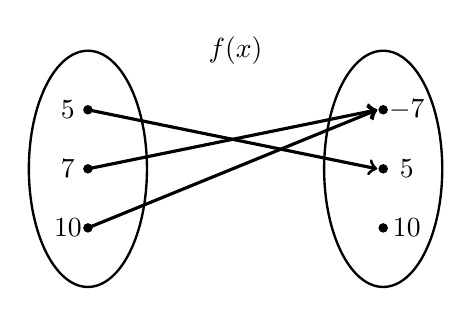
\begin{tikzpicture}[scale=0.75]
	\node at (2.5,2) {$f(x)$};
	% Ellipses
	\draw[line width=0.03cm] (0,0) circle (1 and 2);
	\draw[line width=0.03cm] (5,0) circle (1 and 2);
	
	% Nodes
	\draw[fill=black] (0,1) circle (0.07);
	\draw[fill=black] (0,0) circle (0.07);
	\draw[fill=black] (0,-1) circle (0.07);
	
	\draw[fill=black] (5,1) circle (0.07);
	\draw[fill=black] (5,0) circle (0.07);
	\draw[fill=black] (5,-1) circle (0.07);
	
	% Arrow
	\draw[line width=0.04cm,->] (0,1) -- (4.9,0);
	\draw[line width=0.04cm,->] (0,0) -- (4.9,1);
	\draw[line width=0.04cm,->] (0,-1) -- (4.9,1);
	
	% Labels
	\node at (-0.3,1) {$5\,$};
	\node at (-0.3,0) {$7\,$};
	\node at (-0.3,-1) {$10\,$};
	
	\node at (5.4,1) {$-7$};
	\node at (5.4,0) {$5$};
	\node at (5.4,-1) {$10$};
	\end{tikzpicture}
	\] \pspace


% Problem
\prob Showing all your work, compute the following:
	\begin{enumerate}[(a)]
	\item 150 increased by 42\%
	\item 245 decreased by 20\%
	\item 660 increased by 125\%
	\end{enumerate} \pspace


% Problem
\prob Showing all your work, compute the following:
	\begin{enumerate}[(a)]
	\item 55\% of 143
	\item 1\% of 3.6
	\item 49\% of 49
	\item 121\% of 4000
	\end{enumerate} \pspace


% Problem
\prob Sally Forth is looking to book a vacation trip. She does not want to spend more than \$3,500 on the trip. The prices listed on the travel website she is using to book the trip do not include 7\% sales tax or a \$50 booking surcharge that the website charges (applied to the cost of the trip \textit{before} the tax). What is the highest advertised price on the website that she can book and actually afford? \pspace	


% Problem
\prob Let $M$ represent the total amount of money in your account $d$ days from now. Suppose that right now you have \$15,000 in your account and that you spend \$530 a day.
	\begin{enumerate}[(a)]
	\item Find $M(d)$.
	\item What are the slope and $y$-intercept of $M(d)$? What do they represent?
	\item Find the $x$-intercept of $M(d)$.
	\item Interpret your answer in (c). 
	\end{enumerate} \pspace
	

% Problem
\prob Suppose that you plan on saving \$3,000 to put down on a car. You place \$2,600 into an account which earns 2\% annual interest, compounded quarterly. How long until you have enough money in the account to put down for the car? \pspace
	
	
% Problem
\prob You rent a small studio apartment in NYC for \$3,380 per month to produce social media content. Between hiring actors, purchasing props, travel costs, etc., it costs approximately \$510 to produce a video. However, each video typically makes \$870 in ad revenue and sponsorship deals. Let $C(v)$ and $R(v)$ denote the cost and revenue function to produce $v$~videos. 
	\begin{enumerate}[(a)]
	\item Explain why $C(v)$ and $R(v)$ are approximately linear. 
	\item Find $C(v)$ and $R(v)$. 
	\item What is the minimum number of videos you have to produce to make a profit each month? 
	\end{enumerate} \pspace
	

% Problem
\prob Spencer sold his painting of a man dressed as a T-Rex walking someone else's dog for \$2,427. He places all the money into an account that earns 4.7\% annual interest, compounded quarterly. 
	\begin{enumerate}[(a)]
	\item How long until he has double this amount in savings?
	\item How long until this money in the account has increased in value to \$200,000?
	\end{enumerate} \pspace
	
	
% Problem
\prob Determine if the following function is linear. Explain why or why not.
	\begin{table}[!ht]
	\centering
	\begin{tabular}{c|c}
	$x$ & $f(x)$ \\ \hline
	$0.5$ & $26.45$ \\
	$1.8$ & $21.64$ \\
	$3.9$ & $13.87$ \\
	$4.2$ & $13.44$ \\
	$5.5$ & $7.95$ \\
	$8.1$ & $-1.67$
	\end{tabular}
	\end{table} \pspace	
	
	
% Problem
\prob Consider the linear function $f(x)= \dfrac{4 - 3x}{2}$.
	\begin{enumerate}[(a)]
	\item Find the slope of this linear function. 
	\item Interpret the slope two different ways.
	\item Is the linear function increasing, decreasing, or constant? Explain. 
	\item Determine the $y$-intercept for $f(x)$.
	\item Determine the $x$-intercept for $f(x)$.
	\end{enumerate} \pspace 	
	
	
% Problem
\prob Showing all your work, solve the following equation and verify that your solution is correct:
	\[
	\dfrac{x - 1}{x + 3}= 5
	\] \pspace
	
	
% Problem
\prob A caterer charges a flat fee for each person for whom a meal has to be prepared. The caterer charges \$270 for 15 people and \$360 for 20 people. Let $C(p)$ denote the cost of hiring the caterer to prepare food for $p$ people. 
	\begin{enumerate}[(a)]
	\item Explain why $C(p)$ is linear.
	\item Find $C(p)$.
	\item Interpret the slope of $C(p)$ in the context of the problem. 
	\item Find and interpret $C(32)$. 
	\end{enumerate} \pspace	
	
	
% Problem
\prob Suppose $f(x)$ is the relation given below.
	\[
	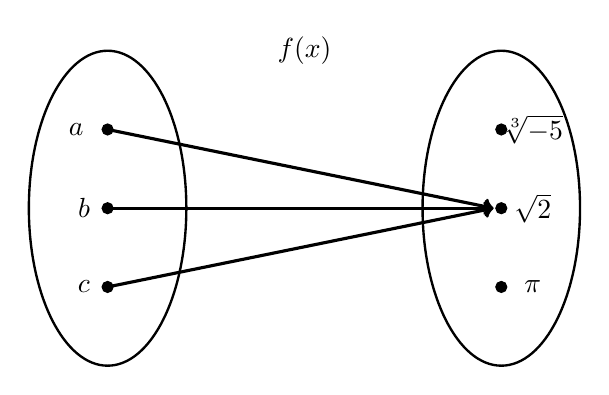
\begin{tikzpicture}
	\node at (2.5,2) {$f(x)$};
	% Ellipses
	\draw[line width=0.03cm] (0,0) circle (1 and 2);
	\draw[line width=0.03cm] (5,0) circle (1 and 2);
	
	% Nodes
	\draw[fill=black] (0,1) circle (0.07);
	\draw[fill=black] (0,0) circle (0.07);
	\draw[fill=black] (0,-1) circle (0.07);
	
	\draw[fill=black] (5,1) circle (0.07);
	\draw[fill=black] (5,0) circle (0.07);
	\draw[fill=black] (5,-1) circle (0.07);
	
	% Arrow
	\draw[line width=0.04cm,->] (0,1) -- (4.9,0);
	\draw[line width=0.04cm,->] (0,0) -- (4.9,0);
	\draw[line width=0.04cm,->] (0,-1) -- (4.9,0);
	
	% Labels
	\node at (-0.4,1) {$a$};
	\node at (-0.3,0) {$b$};
	\node at (-0.3,-1) {$c$};
	
	\node at (5.4,1) {$\sqrt[3]{-5}$};
	\node at (5.4,0) {$\sqrt{2}$};
	\node at (5.4,-1) {$\pi$};
	\end{tikzpicture}
	\]

\begin{enumerate}[(a)]
\item Is $f(x)$ a function? Explain.
\item What is the domain of $f(x)$?
\item What is the codomain of $f(x)$?
\item What is the range of $f(x)$?
\end{enumerate} \pspace
	

% Problem
\prob Do you think a person's height is a function of time? Do you think a peron's salary is a function of their body temperature? For each, explain why or why not. \pspace	
	
	
% Problem
\prob Doug Graves needs to have repairs made to his hearse for his mortuary Look Alive. The reaches out to a bank for a loan to fund the repairs. The bank offers a \$2,500 discount note for 9~months at 9.4\% annual interest.
	\begin{enumerate}[(a)]
	\item How much would Mr. Graves receive from the bank, if he took the loan?
	\item At the end of the 9~months, how much would Mr. Graves owe the bank?
	\end{enumerate} \pspace


% Problem
\prob Ray Gunne is comparing loan rates at two different banks. The first offers loans at a 7.99\% annual interest rate, compounded semiannually, while the other offers a loan at 7.89\% annual interest rate, compounded continuously. Which loan should he take? Justify your answer completely. \pspace	
	
	
% Problem
\prob Tyrell sells mattresses in a store which he rents for \$7500 per month with building costs of approximately \$635 per month. He purchases these mattresses from a distributor at an average cost of \$127 per mattress. On average, each mattress sells for \$547.
        \begin{enumerate}[(a)]
        \item What are Tyrell's fixed costs?
        \item Find $C(m)$, the cost function associated to selling $m$ mattresses. 
        \item Find $R(m)$, the revenue function function for selling $m$ mattresses. 
        \item Without finding $P(m)$, the profit function, find the minimum number of mattresses Tyrell needs to sell each month to make a profit. 
        \end{enumerate} \pspace	
	
	
% Problem
\prob Consider the function given by $\ell(x)= 15x - 60$. 
        \begin{enumerate}[(a)]
        \item Is this function linear? Explain.
        \item Describe the graph of the function.
        \item What is the $x$-intercept for this function? 
        \item What is the $y$-intercept for this function? 
        \end{enumerate} \pspace


% Problem
\prob Consider the linear function $\ell(x, y)= 56.4x - 5.6y$. 
        \begin{enumerate}[(a)]
        \item Explain why this function is linear. 
        \item Find $\ell(10.3, 7.1)$.
        \item What is the slope `in the $x$-direction'? Interpret this slope and indicate whether $\ell$ is increasing or decreasing with respect to $x$. 
        \item What is the slope `in the $y$-direction'? Interpret this slope and indicate whether $\ell$ is increasing or decreasing with respect to $x$. 
        \end{enumerate} \pspace	


% Problem
\prob Let $R(x)$ be the revenue function given by $R(x):= 15.99x$. 
	\begin{enumerate}[(a)]
	\item What is the price per item that the company sets? 
	\item How much revenue is gained by selling 150 items? 
	\item How many items would the company need to sell to make at least \$2,000 in revenue?  
	\end{enumerate} \pspace	
	

% Problem
\prob Let the revenue and cost functions for a company be given by $R(x):= 24.99x$ and $C(x)= 11.20x + 560$. 
        \begin{enumerate}[(a)]
        \item Find the profit function, $P(x)$. 
        \item Find the breakeven point. 
        \item What does the breakeven point represent on the graph of $P(x)$? 
        \item Sketch the functions $R(x), C(x)$ and $P(x)$ along with the breakeven point. 
        \end{enumerate} \pspace

	
% Problem
\prob	 For each of the following, indicate whether the function is linear (T), or not (F). 
	\begin{enumerate}[(a)]
	\item  $y= 4.4x + 50.9$
	\item  $f(x)= x^2 - 2x + 1$
	\item  $w= \frac{5}{6}p + 14$
	\item  $g(t)= \dfrac{t}{t + 1}$
	\item  $r= 16.8(b + 8.3)$
	\item  $h(x)= 6.8x(2.2x + 4.8)$
	\end{enumerate} \pspace	


% Problem
\prob A local radio station charges approximately \$1,800 per advertising slot to local businesses. The building where the radio station is located costs them \$48,000 per month to rent and they pay \$18,360 in electricity each month. Additionally, the cost to pay their employees, cover health insurance, stock the office, purchase and maintain equipment, etc. is approximately \$162,000. Determine the revenue, cost, and profit functions. Then find the equilibrium point. Finally, sketch a plot of all of these in the graph below, being carefully to label your plot and indicate the equilibrium point. 
	\[
	
\begin{tikzpicture}[scale=1.1,every node/.style={scale=0.5}]
	\begin{axis}[
	grid=both,
	axis lines=middle,
	xmin= -1, xmax=15,
	ymin= -1, ymax=15,
	xtick={-1,0,...,15},
	ytick={-15,-14,...,15},
	xticklabels={,,},
	yticklabels={,,}
	]
	\end{axis}
	\end{tikzpicture}
	\] \pspace	
	
	
% Problem
\prob	 Compute the following:
	\begin{enumerate}[(a)]
	\item 83\% of 2,429
	\item 17\% of 94.2
	\item 121\% of 16
	\item 55 decreased by 27\%
	\item 430 increased by 60\%
	\item 38 increased by 130\%
	\end{enumerate} \pspace	
	
	
% Problem
\prob Ira Flatrow wants to buy an antique radio to adorn his fireplace mantel. The radio costs \$849.13. Working for a non-profit, he currently does not have the budget to set aside money each month. Instead, he will invest an up-front amount into an account that earns 3.3\% annual interest, compounded continuously. He hopes that this money will earn enough interest over time so that he will be able to afford the radio. Regardless, he will purchase the radio after 14~months---regardless of whether he has saved enough. If he does not want to spend any extra money at the end of the 14~months, what is the minimum amount he should invest now? \pspace 	
	
	
% Problem
\prob	 A relation $\phi$ is plotted below. 
	\[
	\fbox{
	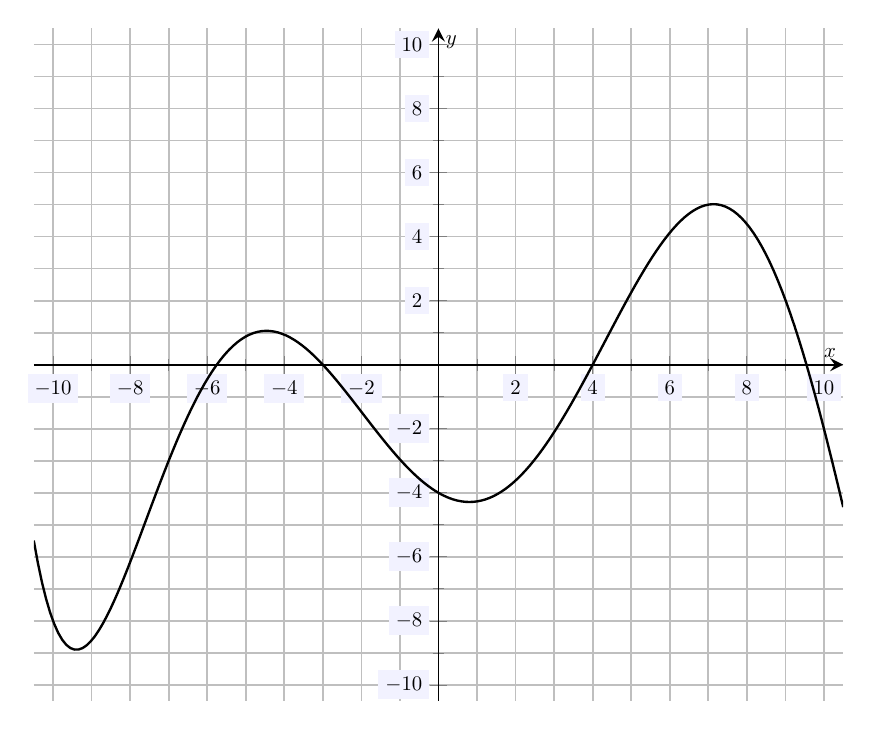
\begin{tikzpicture}[scale=1.5,every node/.style={scale=0.5}]
	\begin{axis}[
	grid=both,
	axis lines=middle,
	ticklabel style={fill=blue!5!white},
	xmin= -10.5, xmax=10.5,
	ymin= -10.5, ymax=10.5,
	xtick={-10,-8,-6,-4,-2,0,2,4,6,8,10},
	ytick={-10,-8,-6,-4,-2,0,2,4,6,8,10},
	minor tick = {-10,-9,...,10},
	xlabel=\(x\),ylabel=\(y\),
	]
	\addplot[line width= 0.02cm,samples=200,domain= -10.5:10.5] ({x},{-4. - 0.695759*x + 0.394934*x^2 + 0.0411407*x^3 - 0.00782987*x^4 - 0.000311831*x^5 + 0.0000378053*x^6}); 
	\end{axis}
	\end{tikzpicture}
	}
	\] 
Using the plot above, answer the following:
	\begin{enumerate}[(a)]
	\item Compute $\phi(9)$.
	\item Find the $y$-intercept for $\phi(x)$. 
	\item Find the $x$-intercepts for $\phi(x)$. 	
	\item As accurately as possible, compute the preimage of $-3$, i.e. $\phi^{-1}(-3)$. 
	\item Explain why (d) implies that $\phi$ does not have an inverse function. 
	\end{enumerate} \pspace
	
	
% Problem
\prob Determine whether the point $(-6, -2)$ is on the graph of $f(x)= 8 - \frac{5}{3}\,x$. Determine also whether the point $(12, -12)$ is on the graph of $f(x)$. For each, explain why or why not. \pspace 	


% Problem
\prob Solve the following equation and verify your solution:
	\[
	4(x - 2)= 5 - 9x
	\] \pspace


% Problem
\prob Is $f(x)= \dfrac{1 - x^3}{x^2 + 5}$ a function? Explain. \pspace 


% Problem
\prob Consider the linear function $f(x)= -3(2x - 7)$. Showing all your work, answer the following:
	\begin{enumerate}[(a)]
	\item Find the rate of change of $f(x)$.
	\item Interpret the rate of change of $f(x)$. 
	\item Determine whether $f(x)$ is an increasing or decreasing function.
	\item Determine the $x$-intercept of $f(x)$.
	\item Find an $x$-value such that $f(x)= 9$.
	\end{enumerate} \pspace


% Problem
\prob Showing all your work, find the solution to the following:
	\[
	\dfrac{5x - 3}{1 - x}= 13
	\] \pspace


% Problem
\prob An oil company is selling off oil in one of their reserves. The amount of oil in the tank in gallons, $O$, after $d$ days is given by $O(d)= 180000 - 19000d$.
	\begin{enumerate}[(a)]
	\item Find and interpret the slope of $O(d)$ in the context of the problem. 
	\item Find and interpret the $y$-intercept of $O(d)$ in the context of the problem. 
	\end{enumerate} \pspace


% Problem
\prob Find the equation of the linear function with slope $-15$ and $y$-intercept 19. \pspace	


% Problem
\prob Suppose you work an hourly job where you are paid \$17.50 an hour. You have already made \$288.75 this week. Let $W$ represent the wages you have been paid by working an addition $h$ hours this week.
	\begin{enumerate}[(a)]
	\item Explain why $W$ is a linear function of $h$. 
	\item Explain why $W(h)= 17.50h + 288.75$.
	\item What is the slope and what does it represent?
	\item What is the $y$-intercept and what does it represent?
	\end{enumerate} \pspace
	

% Problem
\prob	 Richard is a tailor. He uses an automated sewing machine can create custom labels on jackets. Every 4~hours, it is able to stitch 26~jackets. Richard sets the machine going during the night and when he comes in the next morning it has stitched 80~jackets.
	\begin{enumerate}[(a)]
	\item Assuming the machine works at a constant rate, find the number of jackets, $J$, that the machine has stitched $t$~hours from now.
	\item How many total jackets has the machine stitched 8~hours after opening?
	\end{enumerate} \pspace 	
	

% Problem
\prob	 Let $f(x)$ and $g(x)$ be the functions given by the values in the table below. \par
	\begin{table}[H]
	\centering
	\begin{tabular}{r||rrrrr}
	$x$ & $-2$ & $-1$ & $0$ & $1$ & $2$ \\ \hline
	$f(x)$ & $4$ & $5$ & $-1$ & $6$ & $0$ \\
	$g(x)$ & $3$ & $-2$ & $7$ & $0$ & $-1$
	\end{tabular}
	\end{table} \par
Compute the following:
	\begin{enumerate}[(a)]
	\item $f(-2) - g(1)$ 
	\item $(f + g)(0)$
	\item $(fg)(-1)$
	\item $(f \circ g)(2)$
	\item $(g \circ f)(2)$
	\end{enumerate} \pspace
	

% Problem
\prob	 A home was purchased for \$350,000. Unfortunately, home values in the region have depreciated by 1\% per year, every year, for the last 20~years. What is the value of the home now? \pspace
	
	
% Problem
\prob	 Eileen Bach sells propane and propane accessories. She wants to start a YouTube channel where she reviews grills. Of course, she will then have to regularly purchase grills. She wants to review a grill per week and post it to her channel. Eileen estimates that the average grill will cost her \$720. After she is done, she thinks that she will be able to re-sell the grill at a 40\% discount. She plans on saving for 3~months worth of reviews by making a single deposit into an account that earns 1.13\% annual interest, compounded every other month for a period of a year and a half. 
	\begin{enumerate}[(a)]
	\item At the end of the month, how much should Eileen estimate that she has net spent on grills?
	\item How much should she deposit into the account? 
	\end{enumerate} \pspace
	
	
% Problem
\prob	 Pepe Roni owns an Asian fusion restaurant called 9021 Pho. One of the items on the menu has a daily revenue function given by $R(q)= 15.99q$ and a daily cost function given by $C(q)= 5.47q + 287.50$. 
	\begin{enumerate}[(a)]
	\item How much does each item cost to make?
	\item What are the fixed costs for producing this item?
	\item How much is this item sold for?
	\item What is the minimum number of sales of this item that Pepe needs to make in order to turn a profit on its sale?
	\end{enumerate} \pspace
	

% Problem
\prob	 Ty Coon is saving to build a roller coaster park. Though he has investors and can take out loans, he wants to have at least \$26~million saved to bring to the table on his own when the park opens. Ty will deposit money into an account that earns 2.9\% annual interest, compounded continuously. The money will sit for 3~years while the park is being constructed. What is the minimum amount that Ty should deposit now to have at least \$26~million at the end of the three years? \pspace


% Problem
\prob Define what makes a function linear. What `form' does every linear function of one-variable have? \pspace		

% Problem
\prob A linear function has a table whose values are given below. Find the equation of the linear function. Be sure to specify the slope and $y$-intercept.
	\begin{table}[H]
	\centering
	\begin{tabular}{c|c}
	$x$ & $f(x)$ \\ \hline
	$3$ & $5.7$ \\ 
	$4$ & $2.4$ \\
	$7$ & $-7.5$ \\
	$11$ & $-20.7$
	\end{tabular}
	\end{table} \pspace


% Problem
\prob Showing all your work, solve the following equation and verify that your solution is correct:
	\[
	2(1 - x)= 6x + 11
	\] \pspace


% Problem
\prob Jon is paid a base salary of \$56,000 each year. However, he also earns a commission of 2\% of the total amount of sales he makes each year. 
        \begin{enumerate}[(a)]
        \item Explain why Jon's yearly income is a linear function of his sales.
        \item Find a function, $I(s)$, that gives Jon's yearly income, $I$, in terms of his total sales, $s$.
        \item What is the $y$-intercept for this function? What does it represent?
        \item What is the slope for this function? What does it represent? 
        \end{enumerate} \pspace


% Problem
\prob For each of the following, indicate whether the function is linear (T), or not (F). 
	\begin{enumerate}[(a)]
	\item $y= 2x + 1$
	\item $f(x)= 1 - 6x$
	\item $y= x ( 2x + 1)$
	\item $y= 2(x - 1)$
	\item $f(x)= \frac{1}{3}x - 9$
	\end{enumerate} \pspace


% Problem
\prob Complete the following parts: 
        \begin{enumerate}[(a)]
        \item Find the equation of the line through the points $(1, -5)$ and $(-2, 13)$. 
        \item What is the slope and $y$-intercept of the line from (a)? 
        \item Sketch the line from (a) as accurately as possible. 
        \end{enumerate} \pspace


% Problem
\prob Serge is hoping to make an investment in his future by saving his money so that he can one day invest in NFTs. He deposits \$16,000 into an account that earns 2.37\% annual interest, compounded monthly.
	\begin{enumerate}[(a)]
	\item How much does Serge have after 4~years?
	\item Suppose after 2~years, Serge deposits an additional \$4,000 into this account. How much money will he have after four years, i.e. two years after he makes this additional deposit? 
	\end{enumerate} \pspace


% Problem
\prob Showing all your work, compute the following:
	\begin{enumerate}[(a)]
	\item 83\% of 1,295
	\item 3\% of 920
	\item 99\% of 67
	\item 165\% of 81
	\item 20\% of 45.30
	\end{enumerate} \pspace


% Problem
\prob Showing all your work, compute the following:
	\begin{enumerate}[(a)]
	\item 750 increased by 15\%
	\item 60 decreased by 33\%
	\item 840 increased by 92\%
	\item 431 decreased by 99\%
	\item 15 increased by 170\%
	\end{enumerate} \pspace


% Problem
\prob Determine if the relations $f(x)$ and $g(x)$ shown below are functions. Explain why or why not. 
	\[
	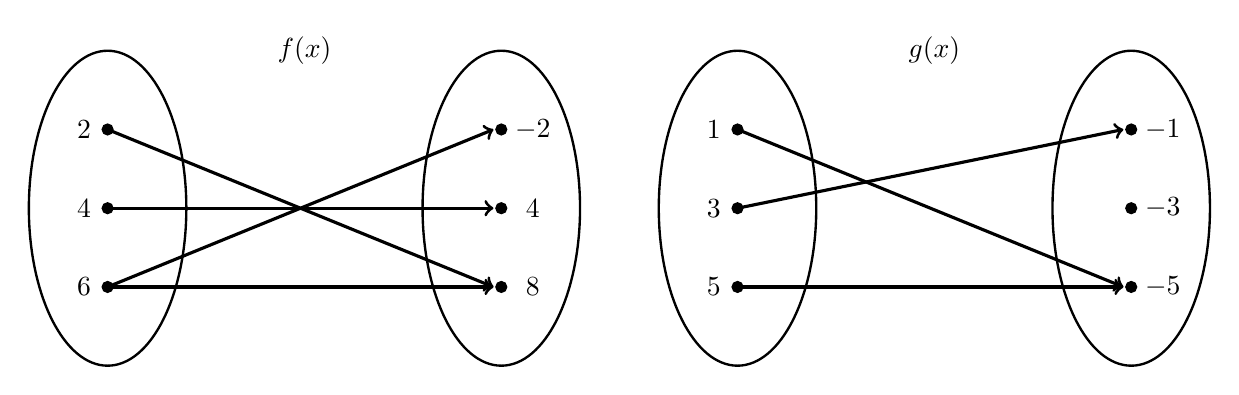
\begin{tikzpicture}
	\node at (2.5,2) {$f(x)$};
	% Ellipses
	\draw[line width=0.03cm] (0,0) circle (1 and 2);
	\draw[line width=0.03cm] (5,0) circle (1 and 2);
	
	% Nodes
	\draw[fill=black] (0,1) circle (0.07);
	\draw[fill=black] (0,0) circle (0.07);
	\draw[fill=black] (0,-1) circle (0.07);
	
	\draw[fill=black] (5,1) circle (0.07);
	\draw[fill=black] (5,0) circle (0.07);
	\draw[fill=black] (5,-1) circle (0.07);
	
	% Arrow
	\draw[line width=0.04cm,->] (0,1) -- (4.9,-1);
	\draw[line width=0.04cm,->] (0,0) -- (4.9,0);
	\draw[line width=0.04cm,->] (0,-1) -- (4.9,1);
	\draw[line width=0.04cm,->] (0,-1) -- (4.9,-1);
	
	% Labels
	\node at (-0.3,1) {$2$};
	\node at (-0.3,0) {$4$};
	\node at (-0.3,-1) {$6$};
	
	\node at (5.4,1) {$-2$};
	\node at (5.4,0) {$4$};
	\node at (5.4,-1) {$8$};
	
	\tikzset{shift={(8,0)}}
	%
	\node at (2.5,2) {$g(x)$};
	% Ellipses
	\draw[line width=0.03cm] (0,0) circle (1 and 2);
	\draw[line width=0.03cm] (5,0) circle (1 and 2);
	
	% Nodes
	\draw[fill=black] (0,1) circle (0.07);
	\draw[fill=black] (0,0) circle (0.07);
	\draw[fill=black] (0,-1) circle (0.07);
	
	\draw[fill=black] (5,1) circle (0.07);
	\draw[fill=black] (5,0) circle (0.07);
	\draw[fill=black] (5,-1) circle (0.07);
	
	% Arrow
	\draw[line width=0.04cm,->] (0,1) -- (4.9,-1);
	\draw[line width=0.04cm,->] (0,0) -- (4.9,1);
	\draw[line width=0.04cm,->] (0,-1) -- (4.9,-1);
	
	% Labels
	\node at (-0.3,1) {$1$};
	\node at (-0.3,0) {$3$};
	\node at (-0.3,-1) {$5$};
	
	\node at (5.4,1) {$-1$};
	\node at (5.4,0) {$-3$};
	\node at (5.4,-1) {$-5$};
	\end{tikzpicture}
	\] \pspace


% Problem
\prob Suppose $f(x)$ and $g(x)$ are the functions given below. 
        \begin{table}[!ht]
        \centering
        \begin{tabular}{| c || c | c | c | c | c | c | c |} \hline
	$x$ & $-3$ & $-2$ & $-1$ & $\phantom{-}0$ & $\phantom{-}1$ & $\phantom{-}2$ & $\phantom{-}3$ \\ \hline
	$f(x)$ & $\phantom{-1}4$ & $\phantom{-}2$ & $\phantom{-}0$ & $-5$ & $\phantom{-}1$ & $\phantom{-}2$ & $\phantom{-}4$ \\ \hline
	$g(x)$ & $\phantom{-1}2$ & $\phantom{-}1$ & $-1$ & $\phantom{-}1$ & $-2$ & $\phantom{-}3$ & $-3$ \\ \hline
	$h(x)$ & $-12$ & $\phantom{-}4$ & $\phantom{-}10$ & $-2$ & $\phantom{-}4$ & $-4$ & $\phantom{-}0$ \\ \hline
        \end{tabular}
        \end{table}

Compute the following: 
        \begin{enumerate}[(a)]
        \item $(f + h)(-1)=$ 
        \item $(h - g)(2)=$ 
        \item $(5f)(2)=$ 
        \item $\left(\dfrac{h}{g}\right)(-3)=$ 
        \item $f(0)\, h(1)=$ 
        \item $g \big(2 - h(1) \big)=$ 
        \item $(f \circ g)(-3)=$ 
	\item $(g \circ h)(3)=$ 
        \item $(h \circ g)(3)=$ 
	\item $(f \circ g \circ h)(0)=$ 
        \end{enumerate} \pspace 


% Problem
\prob Using the plot of the linear function $f(x)$ below, answer the following: 
        \begin{enumerate}[(a)]
        \item Find the slope of the given line.
        \item Find the $y$-intercept of the given line.
        \item Find $f(x)$.
        \item Find the $x$-intercept of $f(x)$. 
        \end{enumerate}
	\[
	\fbox{
	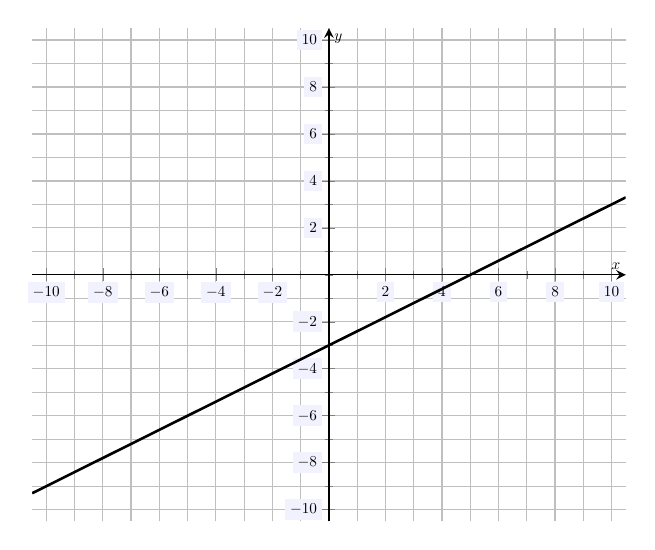
\begin{tikzpicture}[scale=1.1,every node/.style={scale=0.5}]
	\begin{axis}[
	grid=both,
	axis lines=middle,
	ticklabel style={fill=blue!5!white},
	xmin= -10.5, xmax=10.5,
	ymin= -10.5, ymax=10.5,
	xtick={-10,-8,-6,-4,-2,0,2,4,6,8,10},
	ytick={-10,-8,-6,-4,-2,0,2,4,6,8,10},
	minor tick = {-10,-9,...,10},
	xlabel=\(x\),ylabel=\(y\),
	]
	\addplot[domain=-10.5:10.5,samples=2,line width=0.03cm] (x, 3/5*x - 3);
	\end{axis}
	\end{tikzpicture}
	}
	\] \pspace


% Problem
\prob Solve the following equation:
	\[
	3(x - 1)= 1 - 8x
	\] \pspace


% Problem
\prob Explain why $f(x, y)= x^2 - y + 1$ is a function. Then showing all your work, find $f(0, 0)$, $f(0, -4)$, $f(3, 6)$, and $f(-2, 10)$. \pspace 


% Problem
\prob Suppose that the milage of a car, $M$, after $t$~years is modeled by $M(t)= 8500t + 48000$. 
	\begin{enumerate}[(a)]
	\item Find the number of miles on the car after 4~years.
	\item How long until the car's milage is 100,000~miles?
	\end{enumerate} \pspace


% Problem
\prob Find the equation of the line with slope $-\frac{2}{3}$ that passes through the point $(-9 ,10)$. \pspace 


% Problem
\prob Why is 80\% of 485 the same value as the value obtained by reducing 485 by 20\%? Be sure to give an explanation that does not simply involve computing both. Then compute both values as stated. \pspace 


% Problem
\prob Let $\ell(x)= 57.6x - 1654.8$. Explain why $\ell(x)$ is a linear function. Find the $y$-intercept and $x$-intercept of this function. \pspace


% Problem
\prob Suppose that the number of people, $N$ that have ridden the subway $t$~hours after 8:00~am can be modeled by $N(t)= 8429t - 1008$. 
	\begin{enumerate}[(a)]
	\item Find and interpret the slope of $N(t)$.
	\item Does the $y$-intercept of $N(t)$ have an interpretation in the context of this problem? Explain.
	\item Find the number of people that have ridden the subway by 5~pm. 
	\end{enumerate} \pspace


% Problem
\prob Suppose that you take out a loan for \$1,500 at 7.1\% annual interest, compounded daily, for a period of 2~years. Find the amount of interest that you pay on the loan. \pspace 


% Problem
\prob Consider the function $f(x)= 9 - 2x$. 
	\begin{enumerate}[(a)]
	\item Explain why $f(x)$ is a linear function. 
	\item Find the slope and $y$-intercept for $f(x)$. 
	\item Find the $x$-intercept for $f(x)$. 
	\item Find $f(3)$. 
	\item Find an $x$ such that $f(x)= 5$. 
	\end{enumerate} \pspace


% Problem
\prob Susan Flaye has taken out a loan to afford the best possible broom she can to join her local adult Quidditch league. The loan was for \$870 at 9.55\% annual interest, compounded quarterly. She has not made any payments on the loan for the past 2~years. Though Susan has performed fantastically on her team---leading them to over 13 victories---how much does Susan currently owe on her loan? \pspace	


% Problem
\prob Consider the line given by $y= \frac{11}{4}\,x - 6$.
        \begin{enumerate}[(a)]
        \item Put the line in standard form.
        \item Is the point $(-12, -27)$ on the line? Explain.
        \item Is the point $(8, 16)$ on the line? Explain. 
        \end{enumerate}  \pspace


% Problem
\prob Given the following tables, do $f(x)$ and $g(x)$ represent functions? Explain. 
	\begin{table}[!ht]
	\centering \setlength\arrayrulewidth{0.02cm}
	\begin{tabular}{c|ccc|c} 
	$x$ & $f(x)$ & \hspace{2cm} & $x$ & $g(x)$ \\ \cline{1-2} \cline{4-5}
	$1$ & $3$ && $1$ & $4$ \\
	$2$ & $6$ && $2$ & $1$ \\
	$3$ & $9$ && $3$ & $4$ \\
	$4$ & $2$ && $4$ & $5$ \\
	$5$ & $5$ && $1$ & $3$  
	\end{tabular}
	\end{table} \pspace


% Problem
\prob Justin Caese has invested in his future by purchasing the world's largest Pog collection. He currently estimates that the collection is worth \$5,600 and that the value increases each month by 1.17\%.
	\begin{enumerate}[(a)]
	\item How much is the collection worth in 10~years?
	\item How long until the collection is worth \$100,000?
	\end{enumerate} \pspace


% Problem
\prob Given the data in the table below, is it reasonable to say that the data is linear? Explain. 
	\begin{table}[!ht]
	\centering
	\begin{tabular}{c|c}
	$x$ & $f(x)$ \\ \hline
	$1$ & $4$ \\
	$2$ & $6$ \\
	$3$ & $8$ \\
	$4$ & $10$ \\
	$6$ & $12$ 
	\end{tabular}
	\end{table} \pspace


% Problem
\prob Does the formula $f(x):= 2.31x + 9.55$ give a function? Explain. If it is a function, describe its graph. \pspace 


% Problem
\prob Professor Oak is a dendrologist---a scientist who studies woody plants, i.e. trees. He finds that for a certain type of tree, the age of the tree can be closely modeled by the number of rings, $r$, the tree has. He determines that the age of the tree, $A(r)$, in years is approximately given by $A(r)= 15.3r - 6.0$. 
	\begin{enumerate}[(a)]
	\item Is $A(r)$ linear? Explain.
	\item Determine the slope of $A(r)$. Interpret the slope in context. 
	\item Determine the $y$-intercept of $A(r)$. Does the $y$-intercept have an interpretation in context? Explain why or why not. 
	\item For this species of tree, approximate the age of a tree with 11~rings. 
	\end{enumerate} \pspace


% Problem
\prob Showing all your work and explaining your reasoning, answer the following:
	\begin{enumerate}[(a)]
	\item Find the equation of the line through $(-5, 9)$ with slope $-\frac{3}{5}$.
	\item Find the equation of the line through $(0, -4)$ and $(-6, -11)$. 
	\end{enumerate} \pspace
	

% Problem
\prob	 Let $f(x, y)= (x - y)^2 - x + \dfrac{10}{y}$. Find $f(3, -2)$ and $f(4, 5)$. \pspace 


% Problem
\prob Find the equation of the line with $x$-intercept $-7$ and $y$-intercept 3. \pspace 
	
	
% Problem
\prob Suppose $f(x)$ is the function given below.
	\[
	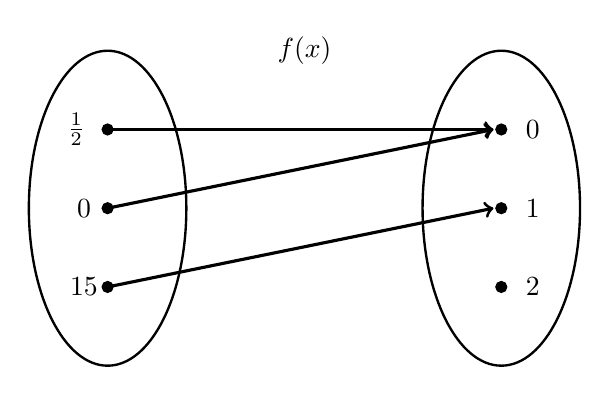
\begin{tikzpicture}
	\node at (2.5,2) {$f(x)$};
	% Ellipses
	\draw[line width=0.03cm] (0,0) circle (1 and 2);
	\draw[line width=0.03cm] (5,0) circle (1 and 2);
	
	% Nodes
	\draw[fill=black] (0,1) circle (0.07);
	\draw[fill=black] (0,0) circle (0.07);
	\draw[fill=black] (0,-1) circle (0.07);
	
	\draw[fill=black] (5,1) circle (0.07);
	\draw[fill=black] (5,0) circle (0.07);
	\draw[fill=black] (5,-1) circle (0.07);
	
	% Arrow
	\draw[line width=0.04cm,->] (0,1) -- (4.9,1);
	\draw[line width=0.04cm,->] (0,0) -- (4.9,1);
	\draw[line width=0.04cm,->] (0,-1) -- (4.9,0);
	
	% Labels
	\node at (-0.4,1) {$\frac{1}{2}$};
	\node at (-0.3,0) {$0$};
	\node at (-0.3,-1) {$15$};
	
	\node at (5.4,1) {$0$};
	\node at (5.4,0) {$1$};
	\node at (5.4,-1) {$2$};
	\end{tikzpicture}
	\]

\begin{enumerate}[(a)]
\item Explain why $f(x)$ is a function.
\item Find the value of $f(x)$ on each value in its domain. 
\item What is the domain of $f(x)$?
\item What is the codomain of $f(x)$?
\item What is the range of $f(x)$?
\end{enumerate} \pspace	
	

% Problem
\prob	 Find the equation of the linear function which passes through the points $(-4, 10)$ and $(6, -8)$. \pspace
	

% Problem
\prob Suppose $f(x)$ and $g(x)$ are the functions given below. 
        \begin{table}[!ht]
        \centering
        \begin{tabular}{| c || c | c | c | c | c | c | c |} \hline
	$x$ & $-3$ & $-2$ & $-1$ & $\phantom{-}0$ & $\phantom{-}1$ & $\phantom{-}2$ & $\phantom{-}3$ \\ \hline
	$f(x)$ & $\phantom{-}0$ & $\phantom{-}5$ & $\phantom{-}4$ & $-1$ & $-5$ & $-1$ & $-3$ \\ \hline
	$g(x)$ & $\phantom{-}1$ & $\phantom{-}2$ & $10$ & $\phantom{-}3$ & $\phantom{-}4$ & $-7$ & $\phantom{-}5$  \\ \hline
        \end{tabular}
        \end{table}

Compute the following: 
        \begin{enumerate}[(a)]
	\item $(f - g)(-1)$
	\item $(fg)(2)$
	\item $(-5g)(-2)$
	\item $(f \circ g)(0)$
	\item $(g \circ f)(0)$
        \end{enumerate} \pspace 	
	

% Problem
\prob Define what it means to be a linear function. Then give an example of a linear function and evaluate it at some value. \pspace 


% Problem
\prob Let $\ell(x)= 18.2 - 13.7x$. Find the slope and $y$-intercept of this function. \pspace 


% Problem
\prob Consider the function $f(x)= 121.5 - 11.6x$. 
	\begin{enumerate}[(a)]
	\item Explain why $f(x)$ is linear.
	\item Find the slope and $y$-intercept of $f(x)$.
	\item Find $f(x)$ when $x= 7.2$
	\end{enumerate} \pspace


% Problem
\prob Suppose that you place \$8,520 into a bank account that earns 1.2\% annual interest, compounded monthly. If you save this money in this bank account for 4~years, how much money do you have at the end of the 4~years? How much interest have you earned? \pspace 	


% Problem
\prob Consider the relation plotted below.
	\[
	\fbox{
	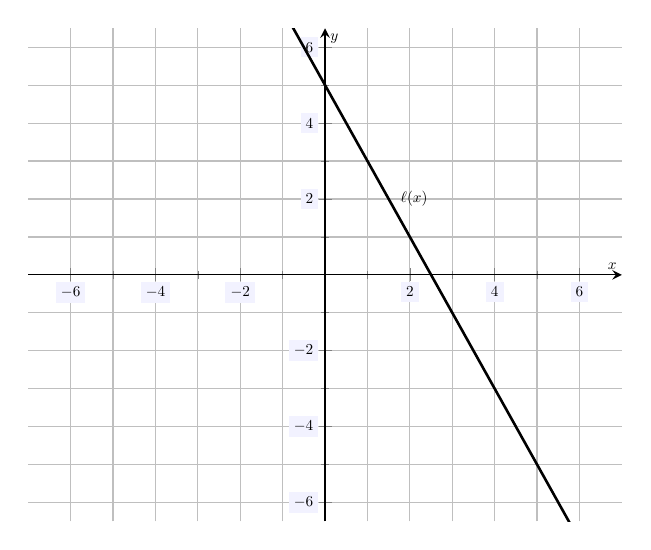
\begin{tikzpicture}[scale=1.1,every node/.style={scale=0.5}]
	\begin{axis}[
	grid=both,
	axis lines=middle,
	ticklabel style={fill=blue!5!white},
	xmin= -7, xmax=7,
	ymin= -6.5, ymax=6.5,
	xtick={-6,-4,-2,0,2,4,6},
	ytick={-6,-4,-2,0,2,4,6},
	minor tick = {-5,-3,...,5},
	xlabel=\(x\),ylabel=\(y\),
	]
	\addplot[domain=-7:7, samples=100,line width=0.03cm] (x,5 - 2*x);
	\node at (2.1,2) {$\ell(x)$};
	\end{axis}
	\end{tikzpicture}
	}
	\]

\begin{enumerate}[(a)]
\item Is $\ell(x)$ a linear function? Explain.
\item Find the equation for $\ell(x)$. 
\item Find the $x$ and $y$-intercepts for $\ell(x)$. 
\item Find a value of $x$ for which $\ell(x)= -3$. 
\end{enumerate} \pspace


% Problem
\prob Explain why $f(x, y)= x^2 - y + 3$ is a function and find the value of $f$ at $(x, y)= (-1, 5)$. \pspace 


% Problem 
\prob Consider the linear function that goes through the points $(-4, 5)$ and $(6, 0)$.
	\begin{enumerate}[(a)]
	\item Find the slope of this linear function.
	\item Find the equation of this linear function.
	\end{enumerate}  \pspace


% Problem
\prob Consider the function given by $W(t)= 568.1 - 13.4t$. 
	\begin{enumerate}[(a)]
	\item Is $W(t)$ a linear function? Explain.
	\item Find the slope of $W(t)$.
	\item Find the $y$-intercept of $W(t)$.
	\item Find the $x$-intercept of $W(t)$. 
	\item Find a value of $t$ for which $W(t)= 100$. 
	\end{enumerate} \pspace


% Problem
\prob Showing all your work, solve the following equation and verify that your solution is correct:
	\[
	5x - 7= 7 - 2x
	\] \pspace
	

% Problem
\prob Donna Mite owns a hair salon called `Hairway to Heaven.' On average, each customer that visits the store spends approximately \$50.97. However, the average cost of serving that customer is approximately \$28.21. The salon has rent and utility costs of approximately \$518.35 to keep open per day. 
	\begin{enumerate}[(a)]
	\item Find the revenue function as a function of the number of daily customers. 
	\item Find the cost function as a function of the daily number of customers. 
	\item What is the minimal number of customers Donna needs to attract to the store each day to turn a profit? 
	\end{enumerate} 
   

\end{document}